\documentclass[dutch,dit,report]{hogentreport}

\usepackage{subcaption}
\usepackage[outputdir=../output]{minted}

\graphicspath{{../images/}}

\addbibresource{voorbeelden.bib}  % Voorbeelden voor het hst over bibliografie
\addbibresource{referenties.bib}  % Referenties in de tekst

\author{Bert {Van Vreckem}, Thomas Aelbrecht, Thomas Parmentier}
\title[Syllabus IT-component]{Research Methods}
\academicyear{2023--2024}

\begin{document}

\maketitle

\chapter*{Voorwoord}
\label{ch:voorwoord}

Deze gids is tot stand gekomen vanuit de begeleiding van de bachelorproef van de opleiding toegepaste informatica aan Hogeschool Gent en werd oorspronkelijk gepubliceerd via Github\footnote{\url{https://github.com/HoGentTIN/bachproef-gids/}}. De bedoeling was om onze studenten wat houvast te geven in hoe ze hieraan in de eerste plaats moeten beginnen, en bevat heel wat tips i.v.m.\ methodologie, werken met {\LaTeX} voor een professionele opmaak, enz.

In het nieuwe curriculum, dat ingevoerd werd vanaf het academiejaar 2020--2021, is er een nieuw opleidingsonderdeel ingevoerd waar we hier expliciet tijd voor kunnen maken. De bachelorproefgids is dan verder uitgewerkt als de cursus voor dat nieuwe vak.

De doelstelling van de bachelorproef binnen onze opleiding is aan te tonen dat je in staat bent om een ``klant'' (binnen de eigen organisatie of extern) \textbf{advies te geven over het in een bedrijfscontext toepassen van een actuele ICT-technologie}. We beogen geen academisch wetenschappelijke studie, maar wel een toegepast onderzoek met voldoende technische diepgang dat een meerwaarde biedt in het gekozen vakgebied.

Dat houdt in dat je aan de slag gaat met een concreet en actueel probleem uit het werkveld. Misschien ben je nog geen expert in dit onderwerp, dus je moet je inwerken door relevante, objectieve en gezaghebbende informatie over dat onderwerp te verzamelen en kritisch te beschouwen. Enerzijds gaat het dan over het opzoeken van bestaande kennis die te vinden is in de vakliteratuur, via experten of belanghebbenden. Anderzijds verwachten we dat tijdens het onderzoek ook nieuwe kennis wordt gecreëerd, bijvoorbeeld via zelf opgezette experimenten, een proof-of-concept of prototype, interviews, enz. Al die informatie moet vervolgens gestructureerd en geanalyseerd worden, in het geval van kwantitatieve gegevens op een statistisch verantwoorde manier. Op basis daarvan kan je een oplossing uitwerken en je advies formuleren voor de klant of opdrachtgever. Dit alles verwerk je in een scriptie die je indient en verdedigt voor een jury.

Hopelijk biedt deze cursus voldoende houvast om je bachelorproef met succes aan te vatten!

\bigskip
Revisie: \today

%---------- Inhoudstafel ------------------------------------------------------

\tableofcontents % Print the table of contents itself

%---------- Corpus ------------------------------------------------------------

\chapter{Een onderzoeksvraag formuleren}%
\label{ch:onderzoeksvraag}

In dit hoofdstuk worden enkele suggesties gegeven voor het zoeken naar een onderwerp. De website van de HOGENT bib heeft daar ook enkele algemene raadgevingen over\footnote{\url{https://bib.hogent.be/how-to/onderwerp-formuleren/inleiding/}}, deze gids is specifiek gericht op de bachelor toegepaste informatica.

Vanuit de opleiding krijgen we van externen regelmatig aanbiedingen van onderwerpen die geschikt zijn voor een bachelorproef, maar dat aanbod is niet groot genoeg om alle studenten van een onderwerp te voorzien. Langs de andere kant is het zelf uitwerken van een onderwerp een interessante kans om je te verdiepen in een onderwerp waar je na je afstuderen graag mee zou verder gaan.

\section{Soorten onderzoek}%
\label{sec:soorten-onderzoek}

Een bachelorproef hoeft geen academische masterthesis proberen na te bootsen. De professionele bachelor heeft zijn eigen waarde het is dus perfect mogelijk om te excelleren binnen de specifieke eigenheid van dit profiel. Het grote verschil bestaat in de eerste plaats uit het soort onderzoek dat gevoerd wordt.

Bij \emph{fundamenteel onderzoek}, dat typisch aan universiteiten uitgevoerd wordt, ligt de nadruk op het uitbreiden van onze kennis in het algemeen. Binnen computerwetenschappen kan het bijvoorbeeld gaan over het ontwikkelen van nieuwe en/of efficiëntere algoritmen voor probleemoplossing. Of de resultaten van fundamenteel onderzoek ook onmiddellijk toepasbaar zijn is van secundair belang.

\emph{Toegepast onderzoek}, daarentegen, probeert een antwoord te formuleren op een concrete vraag uit het werkveld. De onderzoeker zal dan aan de hand van de kennis die er op dit moment beschikbaar is (en gepubliceerd door vakexperten), proberen die vraag te beantwoorden. Dat kan bijvoorbeeld gaan over hoe een nieuwe technologie concreet in een bedrijfscontext kan toegepast worden, een keuze maken tussen verschillende alternatieve producten of technologieën, een vooronderzoek voorafgaand aan het ontwikkelen van een applicatie, enz. Bij toegepast onderzoek is de doelgroep ook heel specifiek, bijvoorbeeld één enkel bedrijf. We merken dan ook dat de onderwerpen die aangebracht zijn door bedrijven ook het best uitgewerkt zijn en het vaakst leiden tot een goede bachelorproef.

\section{Het onderzoeksdomein kiezen}%
\label{sec:het_onderzoeksdomein_kiezen}

Een eerste stap is het kiezen van je onderzoeksdomein. Dit is iets waar eigenlijk niemand je mee kan helpen. Kies een domein waar je zelf in geïnteresseerd bent, zodat je voldoende motivatie kan opbrengen om je je hier in te verdiepen. Je gekozen specialisatierichting in het laatste jaar is wellicht een goed startpunt. In welk soort job zou je na je afstuderen graag starten? Met welke technologieën, platformen, \ldots zou je graag werken?

Ga op zoek te naar de actualiteit binnen je gekozen vakdomein. Belangrijk is je tijd te nemen om je ``onder te dompelen'' in de actualiteit. Dit lukt niet op een avond. Het is efficiënter om hier gedurende een aantal weken regelmatig wat tijd in te steken (bv.\ elke dag een uur). Op de duur zou je in principe de belangrijkste thema's moeten herkennen waar men op dit moment vooral mee bezig is en dat zou inspiratie kunnen geven voor je onderwerp.

In Sectie~\ref{sec:op_zoek_naar_relevante_informatie} vind je enkele concrete tips en startpunten voor het zoeken van relevante informatie.

\section{Onderzoeksvraag en -doelstellingen formuleren}%
\label{sec:onderzoeksvraag_formuleren}

Eens je voeling krijgt met de actualiteit van een onderwerp, leer je typisch ook de belangrijkste problemen en discussiepunten kennen. Die kunnen aanleiding geven tot het formuleren van je hoofdonderzoeksvraag, die je verder kan opsplitsen in concretere deelonderzoeksvragen.

Een goede onderzoeksvraag voor een bachelorproef start vanuit een reële of in elk geval realistische \textit{bedrijfscasus}, een concreet probleem waar een specifiek bedrijf mee worstelt. Dat zorgt meteen ook voor een duidelijke \textit{afbakening} van het onderwerp. Een te vage of algemene onderzoeksvraag leidt nooit tot een goede bachelorproef.

Bijvoorbeeld, ``Wat is de beste agile methodologie voor bedrijven?'' is in dat opzicht \textit{geen} goede onderzoeksvraag. Er zijn verschillende agile methodologieën, en daar is allicht een goede reden voor. Er is geen duidelijke winnaar die voor elk bedrijf het meest geschikt is. Als dat wel zo was, dan zou intussen, een twintigtal jaar na de publicatie van het Agile Manifesto \autocite{BeckEtAl2001}, al duidelijk zijn wat de beste methodologie is. Een geschikte methodologie hangt af van veel factoren: de de bedrijfscultuur, het soort bedrijf, het soort it-oplossingen dat ontwikkeld wordt, de grootte van het bedrijf, enz. Als je je onderzoeksvraag te algemeen formuleert, zal je nooit tot een sluitende conclusie kunnen komen. Dit hebben we in het verleden al te vaak ondervonden. De student schrijft dan in de conclusie ``de beste oplossing hangt af van je voorkeur en je specifieke situatie.'' Met andere woorden, er \textit{is} geen conclusie. Start dus vanuit een concrete casus, bv.\ bedrijf XYZ worstelt met het tijdig en binnen budget opleveren van software en wil een agile methodologie gaan toepassen. Wat is voor hun specifieke situatie de meest geschikte methodologie? Daarmee is het onderwerp duidelijk afgebakend en de meerwaarde ervan is meteen zichtbaar.

Op goede onderzoeksvraag bestaat er nu nog geen sluitend antwoord. Vragen als ``Wat is data mining?'', ``Welke PHP frameworks zijn er?'', ``Wat is de geschiedenis van de Cloud?'' zijn dus niet geschikt, want het antwoord is snel te vinden door even te zoeken op Wikipedia of Google, of door relevante vakliteratuur na te slaan.

Het is ook belangrijk om meteen na te denken over het verwachte resultaat, de \textit{onderzoeksdoelstelling}. Onder welke omstandigheden kan je spreken van een succesvolle bachelorproef? Wat is het concrete eindresultaat dat je wil bereiken?

Voor het formuleren van je onderzoeksdoelstelling (of -doelstellingen) kan je gebruik maken van het S.M.A.R.T.-principe \autocite{UchelenJungjohann2003}:

\begin{description}
  \item[Specifiek] Is de doelstelling eenduidig? Is het duidelijk wie er baat bij heeft?
  \item[Meetbaar] Onder welke (meetbare/observeerbare) voorwaarden of vorm is het doel bereikt? Is het doel om een proof-of-concept of prototype af te leveren? Een analyse voor een te ontwikkelen applicatie? Een vergelijking tussen mogelijke alternatieve oplossingen met een duidelijk advies? Enz.
  \item[Acceptabel] Zijn deze doelen acceptabel voor de doelgroep? Zal de doelgroep de voorgestelde oplossing ook daadwerkelijk kunnen gebruiken?
  \item[Realistisch] Is het doel haalbaar? Is het onderwerp voldoende afgebakend? Is de moeilijkheidsgraad van het probleem op het niveau van de professionele bachelor?
  \item[Tijdsgebonden] Wanneer (in de tijd) moet het doel bereikt zijn? Voor een bachelorproef is dit eenduidig vastgelegd: de deadline voor indienen.
\end{description}

\section{Onderwerp uitschrijven}%
\label{sec:onderwerp_uitschrijven}

Eens je een onderzoeksvraag hebt, kan je je onderwerp uitschrijven om het in te dienen ter goedkeuring. Dat betekent dat je ook al wat literatuuronderzoek gaat uitvoeren. Voor aanwijzingen over de aanpak hiervan, zie Hoofdstuk~\ref{ch:literatuuronderzoek}.

Wat je leest over het onderwerp, moet je dan structureren en formuleren in je eigen woorden in een doorlopende tekst. Een goed hulpmiddel om je gedachten over een onderwerp te ordenen om er later een gestructureerde tekst rond te schrijven is het opzetten van een mindmap. Er bestaan hiervoor verschillende tools die je kosteloos kan gebruiken, zoals bijvoorbeeld XMind\footnote{\url{https://www.xmind.net/}} of FreeMind\footnote{\url{http://freemind.sourceforge.net/}}.

% TODO: voorbeeld mindmap?

In dit stadium is het nog niet de bedoeling een volledig uitgewerkte literatuurstudie uit te schrijven, maar een aantal referenties worden wel verwacht. Je promotor moet na het lezen van je voorstel begrijpen wat de context van je onderzoek is en waarom er een probleem is dat om een oplossing vraagt. Je moet dit kunnen aantonen aan de hand van gezaghebbende vakliteratuur.

Denk ook na over een titel voor je bachelorproef. Die hoeft nog niet definitief te zijn, maar een goede titel maakt duidelijk welke richting je precies wil uitgaan. Een concrete titel geeft je begeleiders het vertrouwen dat je weet wat je precies wil gaan doen en dat dit een realistische doelstelling is. Probeer te letten op het volgende bij het formuleren van een titel:

\begin{itemize}
  \item Formuleer de titel niet als een vraag.
  \item Vermijd obscuur vakjargon en gebruik zeker geen afkortingen. De titel moet ook begrijpbaar zijn voor iemand buiten jouw specifieke vakgebied.
  \item Enkel je vakdomein benoemen is onvoldoende want veel te vaag. Je titel moet concreet zijn en duidelijk maken wat je precies wil onderzoeken. Dat betekent dus ook dat een titel gerust lang mag zijn. Bijvoorbeeld, ``Cloud computing'' is een algemene term die veel ladingen dekt, en die dus niets zegt. ``De selectie van een open source Infrastructure as a Service platform voor het opzetten van een testomgeving voor webontwikkeling'' is een stuk concreter.
\end{itemize}

Bij het beoordelen van een onderwerp, wordt rekening gehouden met volgende criteria:

\begin{itemize}
  \item Er is een concrete, \textbf{duidelijk afgebakende onderzoeksvraag}, onderzoeksdoelstelling.
  \item Het voorstel is \textbf{vernieuwend} en heeft een duidelijke \textbf{meerwaarde} voor een specifieke doelgroep uit het ict-werkveld.
  \item De \textbf{methodologie} is duidelijk verantwoord, onderzoekstechnieken zijn ge\-schikt voor het beantwoorden van de onderzoeksvraag
  \item Er is een duidelijke \textbf{eigen bijdrage} en \textbf{technische diepgang}.
\end{itemize}

\section{Struikelblokken}%
\label{sec:onderwerp-struikelblokken}

Volgende zaken geven ons het idee dat je onderwerp nog onvoldoende is uitgewerkt of dat er nog belangrijke struikelblokken zijn die een succesvolle bachelorproef in de weg staan:


\begin{itemize}
  \item Er is geen concrete reële of realistische \textbf{bedrijfscasus} gekoppeld aan het onderwerp. Onderzoek op bachelorniveau is toegepast, m.a.w.~we proberen concrete, reële problemen op te lossen. Dat moet ook in je onderwerp naar voor komen.
  \item (Eén van) de onderzoeksdoelstelling(en) is \textbf{speculatie over de toekomst} (bv. ``wat zal de impact zijn van het Internet of Things op het dagelijks leven?''). De conclusie van een bachelorproef moet aantoonbaar zijn, toekomstvoorspellingen zijn dat nooit.
  \item Het resultaat van het onderzoek is in grote mate \textbf{afhankelijk van externe factoren}. Als je bijvoorbeeld een enquête zal voeren, is het belangrijk te beseffen dat het niet makkelijk is om voldoende respondenten te vinden. Je zal dus al meteen moeten aangeven op welke manier je van plan bent om een voldoende grote steekproef te nemen. Ook als je plan is om interviews af te nemen bij experten, bedrijven, enz.\ is het belangrijk om al voor de start van je onderzoek de nodige contacten te leggen. Als het immers niet lukt om tijdig de nodige personen te kunnen spreken, komt het resultaat van je bachelorproef in gevaar.
  \item Het onderwerp vertoont onvoldoende \textbf{technische diepgang}. De professionele bachelor toegepaste informatica is een technisch profiel en we verwachten dat je ook aantoont technisch sterk te staan. Een onderwerp als ``wat is de meest gebruiksvriendelijke mobiele applicatie voor thuisbankieren voor senioren?'' voldoet hier bijvoorbeeld \textit{niet} aan. Dit soort applicaties is wordt door banken ontwikkeld en als student zal je nooit toegang krijgen tot de interne werking. Je zal je wellicht moeten beperken tot interviews en/of enquêtes bij de doelgroep. Op deze manier kan je niet aantonen wat je als informaticus in je mars hebt.
  \item De \textbf{referentielijst} is te kort of bestaat uit ongeschikte bronnen. Neem de nodige tijd om een initiële literatuurstudie te voeren en ga verder kijken dan het eerste het beste blogartikel. In Hoofdstuk~\ref{ch:literatuuronderzoek} vind je aanwijzingen om dit aan te pakken.
  \item Het onderwerp ligt \textbf{buiten de scope van een bacheloropleiding of van de student}. Kies een onderwerp dat qua niveau past bij een bacheloropleiding. Een typisch voorbeeld van een te moeilijk onderwerp is \textit{Quantum Computing}, dit is minstens voor een masteropleiding. Een dergelijk onderwerp kan in het oog springen, maar hiermee loop je de kans om in je eigen voeten te schieten qua moeilijkheid.
\end{itemize}

\section{Samenvatting}%
\label{sec:onderwerp_samenvatting}

\begin{itemize}
  \item Neem de tijd om een onderwerp te zoeken dat je ligt.
  \item Bij het uitschrijven van een onderwerp ben je best zo \emph{concreet} mogelijk.
  \item Vermijd struikelblokken als het ontbreken van een concrete casus, speculatie, afhankelijkheid van externe factoren en een te oppervlakkige literatuurstudie.
\end{itemize}

\chapter{Werken met \LaTeX{}}%
\label{ch:voorbereiding}

In dit hoofdstuk behandelen we het opstarten van het werk aan een bachelorproef. Je vindt er enkele aanbevelingen over te gebruiken tools en het onderzoeksproces.

Het is niet de bedoeling dat dit hoofdstuk een {\LaTeX} handleiding wordt, daarvoor zijn er voldoende andere bronnen beschikbaar~\parencite{Oetiker2015}.

We hebben ook een online gids\footnote{\url{https://hogenttin.github.io/latex-hogent-gids/}} samengesteld met de nodige info om met {\LaTeX} aan de slag te gaan, de beschikbare sjablonen conform de HOGENT huisstijl te gebruiken, vaak voorkomende problemen op te lossen, enz. Deze kan je bookmarken en raadplegen wanneer je bijvoorbeeld volgend jaar aan je bachelorproef werkt.

\section{Gebruik van {\LaTeX}}%
\label{sec:gebruik-van-latex}

De meeste studenten zijn gewend om opgemaakte tekst met een klassieke tekstverwerker (typisch MS Word) te schrijven. Voor je bachelorproef is het aangewezen om hier van af te stappen.

Word, zeker met het standaardsjabloon, geeft een layout die niet geschikt is voor publicatie. Functionaliteiten die helpen bij het bewaren van een consistente opmaak (zoals stijlen) zitten verborgen en worden vaak niet gebruikt. Eens de lengte en complexiteit van een Word-document toenemen (en bij een eindwerk is dat zeker het geval), krijg je te maken met inconsistenties in de layout van je tekst, paginanummering, slecht gepositioneerde afbeeldingen, verkeerd opgemaakte bronnenlijst, enz.

Wanneer je niet zorgvuldig te werk gaat bij het kopiëren van tekst vanuit een ander (voorbereidend) document of vanuit een website, wordt de oorspronkelijke layout overgenomen. Als die niet consistent is met deze van je hoofddocument, moet je alles gaan aanpassen. Dit is een bijzonder tijdrovend werk met een grote kans op fouten.

Een klassieke tekstverwerker die gebaseerd is op het WYSIWYG-principe\footnote{\emph{What You See Is What You Get}, d.w.z.\ wat je op het scherm ziet is hoe het er op papier zal uitzien wanneer je het document afdrukt.}, laat je toe om tot in de puntjes te bepalen waar tekst op het papier terecht komt, maar eigenlijk is deze grote vrijheid in dit geval een nadeel. Een strakke en professionele vormgeving is een specialiteit die een grote aandacht voor vaak pietluttige  details vraagt. Dit valt echter buiten onze expertise als informaticus. Wanneer je een significant deel van de tijd bezig bent met het vormgeven van je document, word je bovendien afgeleid van de kern van de zaak: de inhoud van de tekst!

Een ander nadeel van de klassieke tekstverwerker is het binaire bestandsformaat. Dit maakt het onmogelijk om een document in een versiebeheersysteem te steken (zie Sectie~\ref{sec:versiebeheersysteem}). Al gauw gaan er verschillende versies van het document naast elkaar leven: `bachproef 3.docx', `bachproef 5 30 maart.docx', `final draft.docx', `final draft na feedback.docx', `final final draft.docx', `ultimate final draft - this time I mean it.docx', \dots. Je hebt versies op je laptop, op dropbox, op je vaste pc en in je mailbox. Op de duur is het overzicht zoek, vergeet je stukken tekst over te nemen of maak je andere fouten.

Voor het opmaken van een lange tekst met een professionele en strakke vormgeving is {\LaTeX} een aanrader. Dit is \emph{tekstzetsysteem} met een markuptaal (zoals HTML) die ontworpen is voor het op papier zetten van tekst met een opmaak volgens de regels van de kunst. Je schrijft je tekst in de {\LaTeX} markuptaal, en een `compiler' zet deze om in een PDF. Een bijkomend voordel van {\LaTeX} is dat het tekstgebaseerd is, en je het dus kan opslaan in een versiebeheersysteem.

Toegegeven, {\LaTeX} heeft wel degelijk enkele nadelen. Er is een niet te onderschatten leercurve, en zolang je vasthoudt aan de gewoonten die je overgehouden hebt aan het werken met een tekstverwerker, doet {\LaTeX} niet altijd wat je verwacht. Maar je moet de meeste inspanning leveren in het begin, wanneer je {\LaTeX} nog onder de knie moet krijgen. Eens je het basissjabloon met succes kan compileren naar PDF, kan je stelselmatig inhoud toevoegen zonder dat je je nog zorgen hoeft te maken over de vormgeving. Die zal altijd strak en consistent blijven. Zaken zoals hoofdstuk- en paginanummering, verwijzen naar andere hoofdstukken, figuren of bronnen worden automatisch bijgehouden en aangepast wanneer nodig.

Bij het schrijven van een bachelorproef met een tekstverwerker heb je het mees\-te werk op het einde, om alle onvolkomenheden, inconsistenties en fouten in de vormgeving weg te werken. Op dat moment heb je daar meestal niet meer voldoende tijd voor, want de deadline nadert. Het gevolg is vrijwel altijd een document dat onvoldoende afgewerkt is en er heel onprofessioneel uitziet voor de lezer. Dit past niet niet bij een werkstuk dat dient als afsluiter van een \textit{professionele} bacheloropleiding.

Investeer vanaf het begin in het leren van {\LaTeX}, gebruik nooit Word als voorbereiding. Eens je een goed gestructureerd document hebt, en je de basiscommando's onder de knie hebt, kan je je concentreren op inhoud. Als je eerst alles voorbereid in Word om dat pas op het einde, vlak voor de deadline, om te zetten naar {\LaTeX}, zal je veel tijd verliezen met het herstructureren van je document en het leren omgaan met de specifieke eigenschappen van {\LaTeX}.

Wat eventueel wél een nuttige tool kan zijn om nota's en voorbereidende teksten bij te houden is Markdown. Dit is een eenvoudige opmaaktaal die je toelaat om snel geformatteerde tekst te schrijven. Markdown kan je omzetten naar onder andere HTML, PDF, en ook {\LaTeX}, met behulp van Pandoc\footnote{\url{https://pandoc.org}}. Bovendien is Markdown het standaardformaat voor opgemaakte tekst op Github: een document in Markdown dat je op Github bekijkt wordt getoond in een opgemaakte vorm (via een vertaling naar HTML).

\section{Installatie}%
\label{sec:latex-installatie}

Om met {\LaTeX} te kunnen werken heb je het volgende nodig:

\begin{itemize}
  \item Een {\LaTeX} compiler. Afhankelijk van je besturingssysteem zijn de volgende goede keuzes:
  \begin{itemize}
    \item Windows: MiKTeX\footnote{\url{https://miktex.org}} of TeX Live\footnote{\url{https://tug.org/texlive/}}.
    \item macOS: MacTeX\footnote{\url{https://tug.org/mactex/}}.
    \item Linux: TeX Live.
  \end{itemize}
  \item Een {\LaTeX} IDE of editor met goede ondersteuning. Wij raden een van deze aan (omdat ze op alle besturingssystemen goed werken):
  \begin{itemize}
    \item TeXstudio\footnote{\url{https://www.texstudio.org}}.
    \item VS Code met de LaTeX Workshop extensie\footnote{\url{https://marketplace.visualstudio.com/items?itemName=James-Yu.latex-workshop}}.
  \end{itemize}
  \item Een tool voor het bijhouden van bibliografische referenties. Wij raden JabRef\footnote{\url{https://www.jabref.org}} aan (voor alle besturingssystemen). Instructies voor de configuratie vind je in Hoofdstuk~\ref{ch:bibliografie}.
  \item Een {\LaTeX}-sjabloon. Vanuit de opleiding bieden we enkele sjablonen aan:
  \begin{itemize}
    \item Voor de bachelorproef\footnote{\url{https://github.com/HoGentTIN/latex-hogent-bachproef}}
    \item Voor een korte tekst of artikel\footnote{\url{https://github.com/HoGentTIN/latex-hogent-article}} (dit sjabloon gebruik je voor het uitwerken van bachelorproefvoorstel voor Research Methods)
    \item Voor een presentatie\footnote{\url{https://github.com/HoGentTIN/latex-hogent-beamer}}
  \end{itemize}
  \item Lettertypes voor de HOGENT-huisstijl. Deze kan je downloaden en installeren via de Github-repos met de {\LaTeX}-sjablonen\footnote{Bv.\ \url{https://github.com/HoGentTIN/latex-hogent-beamer/tree/main/fonts}}.
  \begin{itemize}
    \item Montserrat (officieel hoofdlettertype van de HOGENT huisstijl)
    \item Code Pro Black (enkel nodig voor de presentatiestijl)
    \item Fira Code (monogespatieerde tekst)
    \item Fira Math (wiskundige formules)
  \end{itemize}
\end{itemize}

Lettertypes installeren kan je op zowel Windows, macOS als Linux door te dubbelklikken op het OTF-bestand en op de knop ``Installeren'' te klikken in het preview-venster. Je kan de bestanden ook rechtstreeks kopiëren naar de directory met lettertypes:

\begin{itemize}
  \item Windows: \verb+C:\Windows\Fonts+ (let er op dat je de lettertypes installeert voor het hele systeem, niet enkel voor de actieve gebruiker!)
  \item macOS: \verb+/Library/Fonts+ of \verb+~/Library/Fonts+
  \item Linux: \verb+/usr/share/fonts+ of \verb+~/.local/share/fonts+
\end{itemize}

\subsection{Installatie op Windows}%
\label{ssec:installatie-op-windows}

Als je de nodige software wil installeren op Windows, dan kan dat makkelijk in een Administrator-console met de package manager Winget:

\begin{minted}[linenos,breaklines,frame=single]{console}
winget install MikTeX.MikTeX
winget install TeXstudio.TeXstudio
winget install Jabref.Jabref
\end{minted}

\subsection{Installatie op macOS}%
\label{ssec:installatie-op-macos}

Ook op macOS gebruik je best een package manager zoals Homebrew\footnote{\url{https://brew.sh}}:

\begin{minted}[linenos,breaklines,frame=single]{console}
brew install --cask mactex
brew install --cask texstudio
brew install --cask jabref
\end{minted}

\subsection{Installatie op Linux}%
\label{ssec:installatie-op-linux}

Linux-gebruikers zijn het meestal gewend om de package manager voor hun specifieke distributie te gebruiken. Op Debian/Ubuntu kan je bijvoorbeeld het volgende commando uitvoeren:

\begin{minted}[linenos,breaklines,frame=single]{console}
sudo apt install texlive-base texlive-latex-base texlive-latex-recommended texlive-bibtex-extra texlive-pictures texlive-fonts-recommended jabref texstudio
\end{minted}

\section{{\TeX}studio configureren}%
\label{sec:texstudio-configureren}

Zoals eerder vermeld raden we {\TeX}studio of VS Code aan als {\LaTeX}-editor. In deze sectie gaan we {\TeX}studio configureren. De configuratie van VS Code is iets complexer en zullen we hier niet behandelen. Kies na opstarten in het menu voor \textit{Options} en vervolgens voor \textit{Configure {\TeX}studio}.

De belangrijkste opties zijn:

\begin{itemize}
  \item Build:
    \begin{itemize}
      \item Default compiler: \textit{XeLaTeX}
      \item Default Bibliography tool: \textit{Biber}
    \end{itemize}
  \item Commands:
    \begin{itemize}
      \item xelatex:
      
        \begin{minted}[autogobble,linenos,breaklines,frame=single]{console}
          xelatex -shell-escape -synctex=1 -interaction=nonstopmode -file-line-error %
        \end{minted}

    \end{itemize}
  \item Editor:
    \begin{itemize}
      \item Indentation mode: Indent and Unindent Automatically
      \item Replace Indentation Tab by Spaces: Aanvinken
      \item Replace Tab in Text by spaces: Aanvinken
      \item Replace Double Quotes: English Quotes: ‘‘’’
    \end{itemize}
  \item Language Checking:
    \begin{itemize}
      \item Default language: selecteer ``nl\_NL-Dutch'' of een gelijkaardige optie voor Nederlands zodat je gebruik kan maken van spellingcontrole. Is deze optie niet beschikbaar? Je kan een woordenboekbestand voor OpenOffice of LibreOffice downloaden en installeren. Het dialoogvenster heeft links die je meteen naar de juiste pagina leiden.
    \end{itemize}
\end{itemize}

\section{Versiebeheersysteem}%
\label{sec:versiebeheersysteem}

Aan een informaticus hoeven hopelijk de voordelen van een versiebeheersysteem niet uitgelegd te worden? Gebruik altijd een versiebeheersysteem zoals Git om je werk bij te houden. Creëer ook een Github repository. Dit is enerzijds een goed backupsysteem (mits je regelmatig synchroniseert met Github), en anderzijds laat het je toe om je werk te delen met je promotor. Eén van de eigenschappen van een versiebeheer is dat het bij uitstek ontworpen is om wijzigingen in \emph{tekstbestanden} op te volgen. Binaire bestandsformaten zoals documenten van een klassieke tekstverwerker zijn hiervoor niet geschikt, wat een extra motivatie is voor het gebruik van \LaTeX{}.

Volgende zaken horen zeker thuis in je repository:

\begin{itemize}
  \item \LaTeX{}-broncode van je onderzoeksvoorstel of de bachelorproef.
  \item in te voegen afbeeldingen.
  \item broncode van zelf geschreven scripts, benchmarks, experimenten, proof-of-concepts, enz. Dit maakt dat je experimenten makkelijker te reproduceren en te valideren zijn door derden.
  \item ruwe resultaten experimenten (in tekstformaat, bv. CSV), transcripties van interviews, enz.
  \item losse nota's, ideeën, enz. Gebruik hiervoor Markdown\footnote{\url{https://guides.github.com/features/mastering-markdown/}} en vermijd Word-do\-cu\-men\-ten.
\end{itemize}

Kortom, \emph{alle} artefacten die resulteren uit je onderzoek horen thuis in de repository. Voor werkdocumenten waar je opgemaakte tekst wenst, maar waarvoor \LaTeX{} overkill is gebruik je Markdown.

Wat hoort \emph{niet} thuis in je repository:

\begin{itemize}
  \item Hulpbestanden aangemaakt bij het compileren van \LaTeX{}. Je kan ervoor zorgen dat deze niet in een repository opgenomen worden door een \texttt{.gitignore}-bestand aan te maken\footnote{Bijvoorbeeld \url{https://github.com/github/gitignore/blob/main/TeX.gitignore}}. Het \LaTeX{}-sjabloon voor de bachelorproef is al goed ingesteld.
  \item Grote (binaire) bestanden zoals ISO's, virtuele machines (bv.\ OVA), enz.
  \item PDFs van de artikels/ebooks die je gelezen hebt (dit wordt beschouwd als ``herdistribueren'' en mag niet onder de auteurswetgeving).
  \item Binaire bestanden die vaak veranderen, bv. Word-documenten.
  \item Bestanden die automatisch gegenereerd worden uit code in Git, bv.\ gecompileerde code.
\end{itemize}

Een versiebeheersysteem wordt pas echt nuttig als je het goed gebruikt. Commit dus zo vaak mogelijk, schrijf duidelijke commit-boodschappen en synchroniseer regelmatig met Github!

Als je een van de HOGENT-sjablonen op Github wilt gebruiken, dan kan je deze best downloaden als ZIP via de groene knop rechtsboven. De repository klonen of een fork aanmaken is in dit geval niet aan te raden. Daarmee neem je immers ook de hele historiek van het sjabloon over en die is niet relevant voor jouw werk. Initialiseer vervolgens zelf een repository met \texttt{git init} en voeg de bestanden van het sjabloon toe met \texttt{git add} en \texttt{git commit}. Vervolgens kan je de repository koppelen aan een nieuwe repository op Github met \texttt{git remote add origin URL} en de inhoud van je lokale repository uploaden met \texttt{git push -u origin main}.

\section{Samenvatting}%
\label{sec:voorbereiding-samenvatting}

De kernpunten van dit hoofdstuk zijn:

\begin{itemize}
  \item Om een strakke, professionele opmaak te bekomen, schrijf je je scriptie beter in {\LaTeX} dan met een klassieke tekstverwerker.
  \item Werk meteen in {\LaTeX}! Ga niet eerst alles voorbereiden in Word en dan pas overzetten.
  \item Gebruik een \emph{reference manager} voor het bijhouden van een bibliografische databank (JabRef is aanbevolen). Zie ook Hoofdstuk~\ref{ch:bibliografie}.
  \item Gebruik een versiebeheersysteem om al je werk in op te slaan (Git is aanbevolen);
\end{itemize}

\chapter{Literatuuronderzoek}%
\label{ch:literatuuronderzoek}

De eerste fase in elk onderzoek is typisch om een overzicht te schrijven van de huidige stand van zaken in het onderzoeksdomein. Daarvoor is het nodig om je te verdiepen in \emph{alles} wat over het onderwerp reeds geschreven is. Dit is het literatuuronderzoek. In elk verslag over onderzoek is het essentieel dat je elke bewering die je doet ook kan aantonen.

Dit hoofdstuk spitst zich in de eerste plaats toe op literatuuronderzoek over een ICT-gerelateerd onderwerp. Wat bereik je precies met een literatuurstudie, hoe kan je er aan beginnen, hoe kan je de bronnen die je vindt gestructureerd bijhouden en op welke manier gebruik je die dan in je tekst? 

In het volgende hoofstuk gaan we in op het correct opmaken van een referentielijst met {\LaTeX} en JabRef (zie Hoofdstuk~\ref{ch:bibliografie}).

\section{Doel van het literatuuronderzoek}%
\label{sec:doel-literatuuronderzoek}

Het belangrijkste doel van een literatuuronderzoek is om vertrouwd te worden met het onderzoeksdomein en die kennis ook door te geven aan de lezers van je bachelorproef. Je gaat dus zoveel mogelijk informatie verzamelen en lezen over het onderwerp zodat je er eigenlijk alles over weet dat er op dit moment over te weten valt. Het is dan de bedoeling om alle voor je onderzoek relevante kennis die je op deze manier hebt opgedaan ook op een gestructureerde manier en in je eigen woorden samen te vatten in een doorlopende tekst. Dit vormt meestal het eerste hoofdstuk (of de eerste hoofdstukken) van je bachelorproef.

De literaturstudie vormt een inleiding op het onderwerp, en bespreekt de huidige stand van zaken. Je introduceert alle relevante vaktermen, vermeldt wat de experten in het domein er over te zeggen hebben en welk onderzoek er in het verleden al eventueel over gedaan is (met uiteraard vermelding van de belangrijkste conclusies). Uit de literatuurstudie moet ook naar voor komen dat er nog hiaten in onze kennis zijn, dat er een probleem is dat om een oplossing vraagt. En dat is uiteraard precies het onderwerp van je bachelorproef.

Op het einde van dit hoofdstuk zou de lezer in staat moeten zijn om de volledige inhoud van je bachelorproef te begrijpen, zonder nog een externe bron te moeten raadplegen. Ga er daarbij van uit dat je bachelorproef gelezen wordt door een ict-professional. Die persoon heeft niet noodzakelijk een achtergrond in het specifieke onderwerp van je bachelorproef, maar heeft wel algemene vakkennis én is typisch geïnteresseerd in de technische details.

\section{Soorten bronnen}%
\label{sec:soorten-bronnen}

In het kader van een onderzoek kunnen we informatiebronnen onderverdelen in deze drie categorieën:

\begin{description}
  \item[Primaire] kennis die je zelf vergaart tijdens je onderzoek. Bijvoorbeeld metingen uit experimenten, resultaten van enquêtes, transcripties van interviews, enz.
  \item[Secundaire] publicatie van kennis, onderzoek, enz.~door anderen. Bijvoorbeeld artikels in vaktijdschriften, boek, presentatie op een conferentie, enz.
  \item[Tertiaire] zoekindexen en encyclopedieën. Bijvoorbeeld Google Scholar, Web of Science, Elsevier ScienceDirect, Arxiv.org, Wikipedia, about.com, Webopedia, Techopedia, Investopedia, enz.
\end{description}

Wanneer in een tekst verwezen wordt naar de literatuur, dan gaat het telkens over \emph{secundaire} bronnen (ook \emph{publicaties} genoemd). Dat betekent ook dat primaire of tertiaire bronnen \emph{niet} kunnen. Er mag dus bijvoorbeeld nooit verwezen worden naar een Wikipedia-artikel, woordenboeken, enz. Tertiaire bronnen zijn wel goede \textit{startpunten} van de zoektocht naar geschikte publicaties.

Een bron moet ook toegankelijk zijn voor de lezer, m.a.w.\ deze moet \textit{gepubliceerd} zijn. Daarom kan je ook \textit{niet} verwijzen naar:

\begin{itemize}
  \item Het verslag van een interview dat je gevoerd hebt, een notitie die je gemaakt hebt tijdens een vergadering, een notitie die je gemaakt hebt tijdens een brainstormsessie, enz.;
  \item Een e-mail die je ontvangen hebt, een chatbericht, een sms-bericht, een tweet, een Facebook-post, enz.;
  \item De syllabus of slides van een cursus die je tijdens je opleiding gevolgd hebt;
  \item Een intern document van het bedrijf dat als opdrachtgever van je onderzoek fungeert.
\end{itemize}

\subsection{De kwaliteit van bronnen beoordelen}%
\label{sub:de-kwaliteit-van-bronnen-beoordelen}

Het is belangrijk om jouw tekst te onderbouwen met bronnen die betrouwbaar en gezaghebbend zijn. Dit is niet altijd makkelijk te evalueren. Veel hangt af van wie de auteur is en welke autoriteit die heeft binnen het vakgebied, wanneer de bron gepubliceerd is, wat de bedoeling was van de publicatie, enz.

Een hulpmiddel bij het beoordelen van een bron is de \emph{CRAAP-test} \autocite{Blakeslee2004}:

\begin{description}
  \item[Currency] of actualiteit: is de bron voldoende recent voor het onderwerp? Let op! Het is niet mogelijk om hier een exact getal op te plakken. Afhankelijk van het onderwerp kan een bron van één jaar geleden al verouderd zijn terwijl een publicatie van twintig jaar geleden nog steeds relevant is!

  \item[Relevance] of relevantie: is de inhoud relevant voor jouw onderzoek? Bevat het informatie die je nodig hebt? Let ook op het doelpubliek. Is het een vakliteratuur, specifiek bestemd voor ict-professionals (dit is waar je naar op zoek bent!), of slechts een populariserende tekst, geschreven voor een groot publiek (deze vermijd je best!)?

  \item[Authority] of autoriteit: is de auteur een autoriteit over het onderwerp? Is het een vakexpert, marketeer, journalist, \ldots? Gaat het over een persoon of een organisatie? In het laatste geval: is de organisatie een overheidsinstantie, een commercieel bedrijf, een non-profit organisatie, een vakorganisatie, \ldots?

  \item[Accuracy] of correctheid: is de bron betrouwbaar? Verwijst de tekst zelf naar bronnen? Zijn de beweringen die gemaakt worden verifieerbaar en goed onderbouwd? Is ook het taalgebruik en de schrijfstijl correct en zakelijk, professioneel?

  \item[Purpose] of doel: wat is de intentie van de tekst? Informeren, aanleren, verkopen, vermaken, onderzoeken, \ldots Wat wil de auteur bereiken? Is de inhoud neutraal of is er een duidelijke mening?
\end{description}

Bij het beoordelen van een bron is het dan noodzakelijk om te weten te komen wie de auteur is en wanneer die geschreven en gepubliceerd is. Van vele websites is dit jammer genoeg niet mogelijk en wordt deze informatie niet gegeven. Dit soort bronnen hoort niet thuis in een literatuurlijst!

\subsection{Publicatievormen}%
\label{sub:publicatievormen}

Kennis wordt doorgegeven en gepubliceerd in verschillende vormen. In deze sectie lijsten we de belangrijkste op en bespreken de betrouwbaarheid en objectiviteit van elk.

Een goede literatuustudie maakt gebruik van een gevarieerde mix van bronnen. Beperk je dus zeker niet tot de eerste de beste zoekresultaten die je via Google gevonden hebt, maar ga actief op zoek naar kwalitatieve vakliteratuur.Over het algemeen getuigt een bronnenlijst met enkel of vooral blogartikels of webpagina's van een zekere gemakzucht!

In de ICT moet je ook rekening houden met het feit dat de meest actuele literatuur in het Engels geschreven is. Enkel Nederlandstalige werken in een bronnenlijst is dus ook een indicatie van een onzorgvuldige aanpak.

\paragraph{Artikel in wetenschappelijk tijdschrift}

Van een artikel, dat in een wetenschappelijk tijdschrift (of Eng. \emph{journal}) gepubliceerd wordt, mag je uitgaan dat er eerst een rigoreus verificatieproces aan vooraf gegaan is. Ingezonden artikels worden door de redacteurs van het tijdschrift doorgegeven aan andere experten in het vakgebied die de verantwoordelijkheid hebben de inhoud ervan op een onafhankelijke en anonieme manier te verifiëren. Dit noemt men in het Engels \emph{peer review}. Dit proces duurt typisch verschillende maanden en kan zelfs uitlopen tot een paar jaar. Publicaties in wetenschappelijke tijdschriften worden algemeen beschouwd als de meest betrouwbare en als er over jouw bachelorproefonderwerp te vinden zijn, is het ten zeerste aan te raden die te lezen. Nadelen is dat het niveau (vooral op vlak van wiskunde) typisch vrij hoog ligt en dus niet altijd even toegankelijk voor de gemiddelde bachelorstudent. Ook is er over sommige, erg praktijkgerichte onderwerpen, geen wetenschappelijke literatuur te vinden.

\paragraph{Artikel in een vaktijdschrift}

Vaktijdschriften zijn gericht op een professioneel publiek, dus dit zijn geen academische, wetenschappelijke teksten. Er gaat ook geen peer review-proces aan de publicatie van artikels vooraf. Typisch beslist een redacteur of een artikel al dan niet gepubliceerd wordt. Vaktijdschriften zijn ook meer en meer enkel online beschikbaar en we rekenen hieronder ook portaalsites rond een bepaald thema of vakgebied, zoals dZone\footnote{\url{https://dzone.com/}}, Informit\footnote{\url{https://www.informit.com/}}, enz.

Het is dan belangrijk te weten wie de auteur van het artikel is. Is dit een erkend vakexpert of een journalist? In het eerste geval is het artikel zeker bruikbaar als bron, maar in het andere moet je er toch eens kritisch naar kijken. Er is immers zelden garantie dat een journalist voldoende expertise in het onderwerp van zijn artikel heeft. Journalisten hebben ook andere drijfveren dan vakexperten en kunnen onder druk staan om een artikel zo te schrijven dat het door zoveel mogelijk mensen gelezen wordt. Soms zullen ze de zaken dan wat sensationeler voorstellen dan ze eigenlijk zijn, of slaan ze de bal mis als het gaat over technische details.

\paragraph{Kranten- of tijdschriftartikel}

Artikels die in kranten of algemene tijdschriften verschijnen zijn in principe minder geschikt als bron voor een bacheloproef in de ict. Ze zijn niet bestemd voor een professioneel publiek, dus ontbreekt de nodige technische diepgang. 

Dit soort artikels is vaak geschreven door journalisten die niet noodzakelijk over de nodige expertise beschikken. Journalisten hebben ook niet de gewoonte om hun bronnen expliciet te vermelden. Het is dan ook belangrijk om kritisch te zijn bij het lezen van dergelijke artikels!

Wanneer je in je tekst een vermelding maakt van een gebeurtenis waar in de actualiteit veel aandacht is voor geweest (bv.\ een cyberaanval, het verschijnen van een revolutionaire nieuwe technologie, product of applicatie, \ldots), dan kan je uiteraard wel verwijzen naar kranten- of tijdschriftartikels die daarover gaan. Je kan dan zelf een kritische beschouwing toevoegen waar het artikel eventueel tekort schoot in het geven van een volledig beeld van de zaak, of waar ze zelfs de bal misgeslagen hebben.

\paragraph{Presentatie op een conferentie}

Zowel de wetenschappelijke als de professionele gemeenschap organiseren wereldwijd conferenties om met elkaar te overleggen, om nieuwe resultaten te presenteren en kennis door te geven. Typisch wordt er enkele maanden voor de start een oproep gedaan om onderwerpen voor presentaties voor te stellen. Bij een wetenschappelijke conferentie wordt dan meestal gevraagd om een uitgeschreven artikel in te dienen dat wordt beoordeeld via een peer-reviewproces dat meestal wel een stuk minder zwaar is dan voor een journal. Voor vakconferenties en voor sommige wetenschappelijke conferenties is een paragraaf tekst met een samenvatting van de inhoud (abstract) voldoende. Bij vakconferenties zal meestal een panel dat door de organisator is samengesteld de inzendingen beoordelen en de presentaties selecteren.

Na afloop van een conferentie wordt de inhoud van de geselecteerde presentaties gebundeld en gepubliceerd. Bij een wetenschappelijke conferentie is dat een {(e-)boek} dat bestaat uit de ingezonden artikels, wat men in het Engels de \emph{proceedings} noemt. Bij een vakconferentie gaat het meestal enkel over de gebundelde presentatieslides, of zetten de sprekers zelf hun slides op een website om presentaties te delen, zoals SlideShare of Speaker Deck. Meer en meer vakconferenties nemen sommige of alle presentaties op en maken die beschikbaar via bv.~Youtube of Vimeo, of via een website in eigen beheer.

Het loont de moeite om uit te zoeken welke conferenties er doorgaan rond het vakgebied waarbinnen jouw gekozen onderwerp past en zo mogelijk de presentaties te bekijken die er zijn doorgegaan.

Qua betrouwbaarheid benadert het niveau van artikels in \emph{conference pro\-ceed\-ings} die van wetenschappelijke artikels in journals. Dit geldt minder voor vakconferenties, omdat er geen peer-review proces aan vooraf gaat. Je kan er wel de belangrijkste experts over een bepaald vakdomein leren kennen en veel bijleren over recente ontwikkelingen binnen het vakgebied.

\paragraph{Thesis, eindwerk}

Thesissen of eindwerken zijn ook vaak interessant als informatiebronnen. De diepgang hangt hier grotendeels af van de opleiding waarvoor de thesis geschreven is: doctoraatsthesis (PhD thesis), masterthesis of bachelorproef. Deze teksten zijn geschreven onder begeleiding van een promotor die borg staat voor de kwaliteit van de inhoud. Als je een gepubliceerde thesis vindt, dan is die dus in principe nagelezen door een expert.

Doctoraatsthesissen staan wat dat betreft ongeveer op het niveau van wetenschappelijke artikels. Meestal is het ook zo dat een of meerdere onderdelen van een doctoraatsthesis ook als artikels in een wetenschappelijk tijdschrift zijn gepubliceerd.

Een masterthesis is geschreven door een student tijdens een masteropleiding, onder begeleiding van een professor of assistent. Je mag er dus van uitgaan dat de inhoud nagekeken is en dat deze voldoende kwaliteit heeft om te worden gepubliceerd. Het moeilijkheidsniveau van een masterthesis ligt meestal een stuk lager dan dat van een doctoraatsthesis.

Misschien bouwt jouw bachelorproefonderzoek verder op een onderwerp dat al eerder is behandeld door een bachelorstudent. Het is sowieso interessant om eens op zoek te gaan of je bachelorproeven van de vorige jaren kan terugvinden over jouw onderwerp. Ook een bachelorproef wordt geschreven onder begeleiding van een promotor, en ook hier geldt dat je er van mag uitgaan dat de inhoud nagekeken is en voldoende kwaliteit heeft om te worden gepubliceerd. Aan HOGENT is het zo dat bachelorproeven die 15/20 of meer halen, worden gepubliceerd via de bibliotheek. Via de bibliotheek kan je dus ook op zoek gaan naar bachelorproeven over jouw onderwerp.

\paragraph{Boek of handleiding}

Over de meeste onderwerpen waarover een bachelorproef toegepaste informatica geschreven wordt, is er wel een boek geschreven. Het is ook belangrijk om de moeite te doen om een boek te lezen over een onderwerp dat je wil behandelen. En boek bevat immers al een gestructureerde samenvatting van de kennis die er over dat onderwerp bestaat. Je vindt er ook vaak definities van vaktermen die je kan gebruiken in je eigen tekst. Soms bevat een boek ook een bronnenlijst die je kan gebruiken om je eigen tekst te onderbouwen.

Ook bij boeken is het belangrijk om te weten wie de auteur is en in hoeverre die de autoriteit heeft om over een onderwerp te schrijven. In principe kan iedereen immers een boek uitgeven, en er is geen formele peer-review, dus geen onafhankelijke validatie van de inhoud.

Bepaalde uitgeverijen zoals O'Reilly, Apress, Pearson, enz.\ staan bekend voor het uitgeven van technische boeken. Deze uitgeverijen hebben een reputatie opgebouwd door alleen boeken uit te geven die voldoen aan een bepaalde kwaliteitsnorm. Ze hebben ook een uitgebreid netwerk van auteurs die zeer bekend zijn in hun vakgebied. Als je een boek van een dergelijke uitgeverij vindt, dan kan je er van uitgaan dat het een degelijk boek is.

Als je tijdens je onderzoek gebruik maakt van specifieke software, of je onderwerp is een vergelijkende studie tussen verschillende applicaties, dan is het belangrijk om de handleidingen van die software te raadplegen, én er ook naar te refereren. Handleidingen worden tegenwoordig meestal online gepubliceerd, maar soms kan je ze ook vinden in de vorm van een boek.

\paragraph{White paper}

Een \emph{white paper} is een rapport over een bepaald onderwerp dat als bedoeling heeft de lezer voldoende achtergrondinformatie te geven over dat onderwerp om het te begrijpen, beslissingen te nemen of een probleem op te lossen. In ons vakdomein worden white papers typisch uitgegeven door bedrijven die een product verkopen gerelateerd aan het behandelde onderwerp. Een bedrijf dat antivirussoftware verkoopt kan bijvoorbeeld white papers uitgeven over het beveiligen van computers, hoe wachtwoorden gekraakt worden, enz.

Het is belangrijk om te beseffen dat white papers meestal niet objectief zijn. De auteurs hebben iets te verkopen, dus het is voor hen belangrijk om het onderwerp op een zodanige manier te presenteren dat het aankopen van hun producten of diensten interessant lijkt. Een leverancier van beveiligingssoftware heeft er bijvoorbeeld belang bij om het probleem van cybercriminaliteit erger voor te stellen dan het in werkelijkheid is. De lezer die ongerust wordt over de toestand is meer geneigd om beveiligingssoftware te kopen.

Lees een white paper dan ook met een zeer kritische blik en tracht ook objectieve informatie uit andere bronnen te vinden.

\paragraph{Blogartikel}

Een blog is meestal (een deel van) een persoonlijke website waar de auteur regelmatig artikels publiceert rond een bepaald onderwerp en haar/zijn kennis deelt met anderen in hetzelfde vakgebied. Over ICT-gerelateerde onderwerpen zijn er duizenden blogs, en de kans is groot dat de belangrijkste experten binnen je gekozen onderwerp er één bijhouden.

Ook bedrijven hebben soms een technische blog waar ze artikels publiceren over problemen of uitdagingen die ze zijn tegengekomen en hoe ze deze aangepakt hebben. Denk bv.\ aan de google Developers Blog\footnote{\url{https://developers.googleblog.com}}, Twitter Engineering Blog\footnote{\url{https://blog.twitter.com/engineering/}}, Netflix Tech Blog\footnote{\url{https://netflixtechblog.com}}, AWS Blog\footnote{\url{https://aws.amazon.com/blogs/}}, \dots

Ook hier is het belangrijk om te achterhalen wie de auteur is en welke autoriteit die heeft over het onderwerp. Wanneer je een artikel vindt over bijvoorbeeld ``continuous delivery'' van Martin Fowler, een wereldwijd erkend expert en spreker rond software-architectuur, dan is dit heel bruikbaar als bron. Een artikel over hetzelfde onderwerp door een andere auteur die bijvoorbeeld na wat zoeken op LinkedIn een marketeer blijkt te zijn, neem je best niet op in je literatuurlijst.

\section{Goede startpunten voor ICT vakliteratuur}%
\label{sec:startpunten-ict-vakliteratuur}

In deze sectie geven we een aantal goede startpunten voor het zoeken naar ICT-gerelateerde vakliteratuur.

\subsection{De HOGENT bib}%
\label{ssec:hogent-bib}

De HOGENT bib heeft als taak om kwalitatieve informatiebronnen beschikbaar te maken voor onderzoekers, docenten en studenten. Ga dus zeker naar de website\footnote{\url{https://www.hogent.be/student/bibliotheken/}} kijken of ga persoonlijk langs en vraag de medewerkers om raad.

Je kan eerst en vooral zoeken in de catalogus van de bibliotheek zelf. De kans is eerlijk gezegd relatief klein dat je op deze manier een relevant en voldoende recent boek vindt, maar wat je op deze manier wél kan vinden is bachelorproeven over jouw onderwerp die al eerder geschreven zijn. Deze proeven zijn een goede bron van inspiratie en kunnen je helpen om je eigen onderzoeksvraag af te bakenen of om er op verder te bouwen.

Verder kan je ook zoeken naar vaktijdschrijften of externe databanken voor vakliteratuur. De bib heeft een abonnement op een aantal van deze databanken, en je kan er als student gratis toegang toe krijgen. Verderop geven we enkele goede databanken voor ICT-gerelateerde vakliteratuur.

Een abonnementen tot zo'n databank wordt automatisch geactiveerd als je op het campusnetwerk zit. Dat betekent dat je vanop de campus in principe nergens hoeft in te loggen om toegang te krijgen en dat je publicaties meteen kan downloaden als PDF, EPUB, enz.

Als je thuis of een andere locatie aan het werk bent, dan kan je VPN aanzetten zodat het lijkt alsof je op de campus zit. De website van de IT-helpdesk geeft instructies over hoe je de VPN-client moet installeren.

Een andere mogelijkheid is om met je HOGENT-emailadres en wachtwoord in te loggen op de website van Academic Software\footnote{\url{https://www.academicsoftware.eu/}}, en in het aanbod te zoeken naar ``BIB bronnen HOGENT''. Selecteer de HOME USE-versie en klik op Starten. Er zal een nieuw tabblad geopend worden met wat lijkt op een webbrowser binnen jouw webbrowser met de hoofdpagina van de HOGENT-bib. Dit is effectief een virtuele omgeving die vanop de campus wordt opgestart en van waar je dus de volledige toegang hebt tot alle databanken. Je kan ook via deze weg publicaties downloaden naar je eigen pc. Deze werkwijze is iets omslachtiger in gebruik dan VPN, maar je hoeft er niets voor te installeren.

\subsection{Startpunten voor ``wetenschappelijke'' literatuur}%
\label{ssec:startpunten-wetenschappelijke-literatuur}

De professionele bacheloropleiding toegepaste informatica is vooral een technische en praktijkgerichte opleiding en niet zozeer een academische. Toch mag je als ict'er academische, wetenschappelijke bronnen niet uit de weg gaan. Nu zal je voor het ene vakgebied (zoals data engineering) ongetwijfeld meer academische literatuur vinden dan het andere (zoals mobiele applicatieontwikkeling), maar doe in elk geval een poging!

Als je op zoek bent naar wetenschappelijke literatuur, dan kan je beginnen met de volgende startpunten:

\paragraph{Google Scholar}

Google Scholar\footnote{\url{https://scholar.google.com/}} is een zoekmachine die zich richt op wetenschappelijke literatuur. Je kan er zoeken naar artikels die verschenen zijn in wetenschappelijke journals of gepresenteerd op conferenties (InProceedings) boeken, proefschriften, enz. Als je vanop de campus of via VPN werkt, dan word in de zoekresultaten meteen getoond of de publicatie beschikbaar is via een van de abonnementen van de HOGENT bib. Je ziet dit aan de links met de tekst ``[Fulltext@HOGENT]''.

\paragraph{Elicit}

Elicit\footnote{\url{https://www.elicit.be/}} is een AI assistent die je kan helpen bij het zoeken naar wetenschappelijke literatuur. Je kan er vragen stellen in natuurlijke taal, en Elicit zal je een lijst van relevante publicaties tonen. Elicit is vooral handig als je een onderwerp wil verkennen en niet precies weet waar je moet beginnen.

\paragraph{Elsevier ScienceDirect}

Elsevier is één van de grootste uitgeverijen van wetenschappelijke publicaties. ScienceDirect\footnote{\url{https://www.sciencedirect.com}} is een zoekmachine in hun catalogus van journals, conference proceedings, enz. Ook hier krijg je meteen toegang tot de volledige tekst vanaf de campus of via VPN. ScienceDirect bevat een grote hoeveelheid publicaties over ict en computerwetenschappen.

\paragraph{Springer Link}

Springer is een andere grote uitgeverij van wetenschappelijke publicaties. Springer Link\footnote{\url{https://link.springer.com/}} is de zoekmachine voor hun catalogus. Deze is bij uitstek interessant voor informatici omdat ook de boeken van de uitgeverij Apress langs deze weg toegankelijk zijn. Daarover later meer.

\paragraph{Andere (commerciële) databanken}

Er bestaan nog andere databanken, maar deze zijn ofwel veel breder dan enkel ict, of de HOGENT bib heeft er geen abonnement voor:

\begin{itemize}
  \item Web of Science\footnote{\url{https://www.webofscience.com/}} is zo'n brede databank (mét abonnement).
  \item Via IEEE Explore\footnote{\url{https://ieeexplore.ieee.org}} van het Institute of Electrical and Electronics Engineers (IEEE, een vakorganisatie) kan je ook enorm veel artikels over computerwetenschappen vinden. Jammer genoeg heeft HOGENT hier \textit{geen} abonnement voor en zijn vele bronnen niet beschikbaar voor ons.
  \item ACM Digital Library\footnote{\url{https://dl.acm.org}} van de Association for Computing Machinery, is eveneens een relevante databank die je ongetwijfeld zal tegenkomen in zoekresultaten, maar waar we geen toegang toe hebben.
\end{itemize}

Via de website van de HOGENT bib kan je nog meer databanken vinden: klik op de homepagina van de bib op ``Databanken'', en dan onder de kop ``Overzicht databanken per departement'' op ``IT en Digitale Innovatie'' en ``Toegepaste informatica''. Let er wel op dat deze soms zeer breed zijn, niet echt gericht op ict of minder geschikt als bron voor een bachelorproef (bv.\ LexisNexis, een databank van kranten en nieuwsmagazines).

\paragraph{Open Access bronnen}

De hierboven genoemde databanken zijn in principe niet gratis (hoewel je als student wel gratis toegang krijgt als de HOGENT bib een abonnement heeft). Als je op zoek bent naar open access publicaties, dan kan je beginnen met de volgende startpunten:

\begin{itemize}
  \item arXiv\footnote{\url{https://arxiv.org}}: een online archief waar veel auteurs in de exacte wetenschappen (o.a.\ computerwetenschappen) hun artikels publiceren voordat ze ze indienen bij een journal, dus vóór het peer-reviewproces.
  \item CiteSeerX\footnote{\url{https://citeseerx.ist.psu.edu}}: een publieke zoekmachine en digitaal archief voor academische artikels, vooral in computerwetenschappen, opgezet door Pennsylvania State University.
  \item Internet Archive Scholar\footnote{\url{https://scholar.archive.org}}: een zoekmachine naar academische literatuur onderhouden door het Internet Archive.
\end{itemize}

Open acces betekent dus dat iedereen vrij toegang heeft tot de publicatie, zonder abonnement. Recentelijk zijn de grote uitgeverijen als Elsevier en Springer onder vuur te komen liggen omwille van hun verdienmodel. Enerzijds betalen universiteiten en hogescholen hoge bedragen voor hun abonnementen, maar anderzijds moeten ook onderzoekers die een artikel willen publiceren daarvoor betalen. Uitgeverijen organiseren weliswaar het administratieve aspect van het peer-reviewproces, maar uiteindelijk besteden ze dat uit aan academici, vakexperten die hier niet voor vergoed worden. Op die manier slaagden uitgeverijen er in om hun winstmarges enorm te laten toenemen. 

Vele onderzoekers worden gesubsidieerd door overheden en dus onrechtstreeks ook door de belastingbetalers. Zij vinden dat het resultaat van hun onderzoek ook toegankelijk moet zijn voor diegenen die het mogelijk maakten en dat de grote uitgevers onredelijk grote winsten maken zonder zelf een significante meerwaarde te creëren.

Enkele activisten gingen zelfs een stuk verder dan openlijk protesteren tegen deze gang van zaken. In 2010 schreef Aaron Schwarz een script waarmee systematisch artikels gedownload werden van JSTOR, een online archief met betalende toegang, via een gastaccount dat hij van het MIT ter beschikking had gekregen. Zijn arrestatie en de daarop volgende dreiging van een monsterboete en een 35-jarige gevangenisstraf dreven hem in 2013 tot zelfmoord. In 2011 startte de Kazachstaanse Alexandra Elbakyan de site Sci-Hub, een digitaal archief met zoekmachine voor artikels die in principe achter een ``paywall'' zitten. Op dit moment zouden er een 90-tal miljoen bestanden in het archief zitten. In de academische wereld kan het initiatief op vrij grote steun rekenen, maar uiteraard leidde dit ook tot rechtzaken, o.a.\ in de VS en India. In sommige landen, waaronder België, moeten ISP's de DNS-naam van de site blokkeren en bezoekers van de site omleiden naar een webpagina met een melding van de politie.

In elk geval, open access is een groeiende trend en meer en meer academische instituten kiezen er expliciet voor om enkel te publiceren in journals met open access tot de gepubliceerde artikels.

\subsection{Startpunten voor technische vakliteratuur}%
\label{ssec:technische-vakliteratuur}

Niet voor elk mogelijk onderzoeksdomein van een bacheloproef bestaan er ook effectief \textit{wetenschappelijke} publicaties. Maar wat je zeker wél zou moeten vinden is \textit{vakliteratuur}, geschreven voor en door ict-specialisten. Je zou op zijn minst één of enkele boeken over het onderwerp van je bachelorproef moeten zoeken en lezen!

Hier vind je enkele nuttige startpunten:

\paragraph{Springer Link}

Springer Link hebben we al eerder vernoemd in het kader van wetenschappelijke literatuur. Maar via deze weg kan je ook de catalogus van uitgeverij Apress raadplegen, waar je vele ict-gerelateerde boeken kan terugvinden. Vanop de campus of via VPN kan je deze als PDF of EPUB gratis downloaden.

\paragraph{EBSCOhost}

Packt Publishing is een gelijkaardige uitgeverij met een grote hoeveelheid boeken over ict. Via EBSCOhost\footnote{\url{https://search.ebscohost.com/login.aspx?authtype=ip,uid&custid=s4061053&groupid=main&profile=ehost&defaultdb=nlebk} (zal enkel werken op de campus of via VPN)} (waarop de HOGENT bib een abonnement heeft) kan je deze eveneens downloaden als PDF of EPUB.

\paragraph{Vakconferenties}

Steeds vaker worden lezingen op vakconferenties opgenomen en publiek toegankelijk gemaakt via Youtube, Vimeo, Slideshare, enz. Ga dus op zoek naar de namen van conferenties binnen jouw specifieke vakgebied (bv.\ Configuration Management Camp, FOSDEM, Google IO, Monitorama, OSCON, Velocity, WWDC, \ldots) en kijk eens of je presentaties terugvindt die relevant zijn voor jouw onderzoek.

\paragraph{Vaktechnische websites}

Enkele websites streven er naar om online communities te vormen onder ict professionals en het publiceren van technische artikels over actuele onderwerpen. Deze zijn typisch geschreven door vakspecialisten en worden onderworpen aan een peer-re\-view\-pro\-ces voor publicatie. Op die manier nemen ze de plaats in van ``klassieke'' gedrukte vaktijdschriften.

DZone\footnote{\url{https://dzone.com/}} en InfoQ\footnote{\url{https://www.infoq.com}} zijn voorbeelden van dit soort websites. Je vindt er aparte rubrieken voor de grote deeldomeinen van ict, bv.\ software-architectuur en -ont\-wik\-ke\-ling, databases, netwerken, DevOps, cybersecurity, \ldots

\paragraph{Online leeromgevingen en cursussen}

Als het onderwerp van je bachelorproef gaat over een domein waar je nog niet zo veel van weet, dan is het misschien nuttig om er een cursus over te volgen. Tegenwoordig kan je over de meest uiteenlopende onderwerpen (in het bijzonder over ict) een online cursuss of MOOC (massive open online course) volgen. Vaak zijn die betalend, maar sommige zijn gratis of kan je als student van HOGENT gratis volgen. Enkele ideeën:

\begin{itemize}
  \item Cisco Networking Academy\footnote{\url{https://www.netacad.com}}: via de opleiding heb je misschien al een account. Je kan langs deze weg ook inschrijven voor andere cursussen dan deze die binnen de opleiding gebruikt worden.
  \item Coursera\footnote{\url{https://www.coursera.org}}, een MOOC provider die samenwerkt met zowel universiteiten als grote it-bedrijven met zowel gratis als betalende cursussen.
  \item The Cyber Mentor\footnote{\url{https://www.thecybermentor.com}}: cybersecurity, ethical hacking
  \item edX\footnote{\url{https://www.edx.org}}, een MOOC provider gecreëerd door MIT en Harvard met zowel gratis als betalende cursussen.
  \item LinkedIn Learning\footnote{\url{https://www.linkedin.com/learning/}}: gratis toegang via Academic Software.
  \item Microsoft Learn\footnote{\url{https://learn.microsoft.com/}} (het vroegere Technet)
\end{itemize}

%% TODO: cursussen die niet publiek toegankelijk zijn (bv. cursus van de opleiding toegepaste informatica aan HOGENT) zijn niet geschikt als bron. Iemand die niet ingeschreven is voor die cursus heeft er immers geen toegang toe.

\section{Samenvatting}%
\label{sec:literatuuronderzoek_samenvatting}

\begin{itemize}
  \item Het doel van de literatuurstudie is om jezelf en de lezer van je bachelorproef voldoende context te geven om het onderwerp ten gronde te begrijpen.
  \item Er zijn drie soorten bronnen: primaire (resultaten van eigen onderzoek), secundaire (publicaties in wetenschappelijke of vakliteratuur) en tertiaire (encyclopedieën en zoekindexen). In een bibliografie horen enkel \emph{secundaire} bronnen thuis.
  \item Het is belangrijk om bronnen kritisch te beoordelen. Gebruik de CRAAP-test!
  \item Gebruik niet enkel Google als startpunt voor je zoektocht, maar gebruik zoekmachines specifiek voor wetenschappelijke en vakliteratuur. Zorg voor variatie in je bronnen! Dus niet enkel blogs of webpagina's, maar zeker ook boeken, technische of wetenschappelijke artikels, enz.
\end{itemize}


% \section{Op zoek naar relevante informatie}%
% \label{sec:op_zoek_naar_relevante_informatie}

% Via de HOGENT bib krijg je toegang tot een grote hoeveelheid wetenschappelijke en vakliteratuur die niet publiek beschikbaar zijn. Dit gaat veel verder dan de boeken die in de bib beschikbaar zijn. Daarnaast zijn immers nog elektronische bronnen (ebooks, tijdschriften, enz.) te raadplegen. Ook (goede) bachelorproeven van vorige jaren kan je op deze manier vinden. De catalogus is te raadplegen via \url{https://www.hogent.be/student/bibliotheken/}.

% Databanken die niet publiek beschikbaar zijn kan je raadplegen als je op de campus bent, of thuis via de HOGENT VPN. Voor ons vakgebied zijn in het bijzonder volgende databanken interessant:

% \begin{itemize}
%   \item Elsevier ScienceDirect
%   \item Springer Online Journals
%   \item Web of Science
%   \item Google Scholar
% \end{itemize}

% Google Scholar is een zoekmachine voor wetenschappelijke literatuur die zowel in publiek toegankelijke (``open access'') als betalende publicaties zoekt. Als je Scholar gebruikt vanop de campus of via de VPN, krijg je automatisch toegang tot de publicaties waarop de HOGENT bib een abonnement heeft.

% Andere, publiek toegankelijke startpunten voor het zoeken:

% \begin{itemize}
%   \item Arxiv.org is een database van Open Acces artikels in een hele reeks onderzoeksdomeinen, o.a.\ de Computing Research Repository\footnote{\url{http://arxiv.org/corr/home}}.

%   \item Ook Wikipedia is een goed startpunt voor je onderzoek, maar vergeet niet dat Wikipedia-artikels op zich niet kunnen als referenties. Lees dus de oorspronkelijke bronnen van het artikel na en gebruik die als ze relevant zijn voor je bachelorproef.

%   \item Er bestaan verschillende portaalsites voor actuele ict-gerelateerde onderwerpen waar technische artikels, presentaties, interviews, enz.\ op verschijnen, bv.\ dzone.com\footnote{\url{https://dzone.com/}}, infoq.com\footnote{\url{https://www.infoq.com/}}, enz.

%   \item Ga op zoek naar voor je vakgebied relevante conferenties, workshops, symposia, enz. Je hoeft je daarbij niet te beperken tot conferenties in eigen land! Voorbeelden zijn Devoxx\footnote{\url{https://devoxx.be/}} (Java), Google IO\footnote{\url{https://events.google.com/io2016/}} (Android), WWDC\footnote{\url{https://developer.apple.com/wwdc/}} (iOS), Configuration Management Camp\footnote{\url{http://cfgmgmtcamp.eu/}} (Linux Systeembeheer), enz.

%         Meer en meer worden de lezingen van conferenties gefilmd en gepubliceerd op Youtube of Vimeo\footnote{Voor Devoxx bijvoorbeeld op \url{https://www.youtube.com/channel/UCCBVCTuk6uJrN3iFV\_3vurg}}. Je kan ook de sprekers opzoeken en nagaan of ze hun slides gepubliceerd hebben op Slideshare\footnote{\url{https://slideshare.net/}} of Speakerdeck\footnote{\url{https://speakerdeck.com/}}.

%   \item Zijn er lokaal verenigingen die geïnteresseerd zijn in je vakgebied? Bijvoorbeeld OWASP Belgium\footnote{\url{https://www.owasp.org/index.php/Belgium}} (beveiliging van mobiele en webapplicaties). Je kan naar zulke groepen zoeken via Meetup\footnote{\url{https://meetup.com/}} of ook via LinkedIn\footnote{\url{https://www.linkedin.com/}} (zoek specifiek naar groepen zoals het Belgian IT Infrastructure Network\footnote{\url{https://www.linkedin.com/groups/2092569}}). Kijk eens na of er binnenkort evenementen in de buurt zijn en ga er naartoe.

%   \item Wie zijn de belangrijkste namen in de ``community''? Keynote-speakers op conferenties, auteurs van de belangrijkste boeken over het onderwerp, enz. Volg deze personen op Twitter, zoek uit of ze een blog hebben, actief zijn op LinkedIn, enz. Lees al wat je kan vinden dat ze geschreven hebben de laatste jaren.

%   \item Zoek uit of er nieuwsbrieven bestaan over je onderwerp, die periodiek updates uit sturen over de actualiteit binnen dat vakgebied. Voorbeelden zijn Cron.Weekly\footnote{\url{https://www.cronweekly.com/}} (Linux systeembeheer), DevOps Weekly\footnote{\url{http://www.devopsweekly.com/}} of JS Weekly (en aanverwanten)\footnote{\url{https://javascriptweekly.com/}}.
% \end{itemize}
\chapter{Een bibliografische databank bijhouden}%
\label{ch:bibliografie}

In het vorige hoofdstuk (zie Hoofdstuk~\ref{ch:literatuuronderzoek}) hebben we besproken hoe je gericht op zoek kan gaan naar ict-gerelateerde vakliteratuur. Het is belangrijk om alle informatie die je op die manier gevonden hebt op een gestructureerde manier bij te houden, zodat je bij het schrijven van je scriptie of paper kan verwijzen naar je bronnen en zodat je de referentielijst of bibliografie kan opmaken. Hoe je dat aanpakt kom je te weten in dit hoofdstuk.

Het verwijzen naar bronnen en opmaken van een bibliografie moet op een strakke, strikt vastgelegde manier gebeuren. Hiervoor bestaan verschillende stijlen, bv.\ de Chicago Manual of Style, IEEE, American Psychological Association (APA), enz. Op HOGENT is gekozen voor de APA-stijl\footnote{Zie cursus \emph{Kritisch Denken en Onderzoekscompetenties voor de Bachelorstudent} op Chamilo}, wellicht de belangrijkste standaard voor publicaties in het domein van de sociale wetenschappen. Het gebruik ervan is dus verplicht voor alle scripties en papers in alle opleidingen van de hogeschool. Dat geldt zowel voor de opmaak van de literatuurlijst als refereren naar bronnen in de tekst.

De opmaakregels voor referenties en bibliografieën in de APA-stijl zijn uitgebreid en vrij complex. Gelukkig hoeven we dit niet volledig manueel te doen. Er bestaan softwarepakketten die dit grotendeels automatiseren: bibliografische databanken of (in het Engels) \emph{reference management software}.

\section{Bibliografische databank}%
\label{sec:bibliografische-databank}

Een bibliografische databank laat je toe metadata over de gelezen werken gestructureerd bij te houden: titel, auteur, jaartal, en dergelijke, maar ook (aanklikbare) URLs, PDFs van artikels, nota's, enz.

In de cursus \emph{Kritisch Denken en Onderzoekscompetenties voor de Bachelorstudent} wordt gesuggereerd om Endnote te gebruiken als bibliografische databank. Het nadeel hiervan is dat dit een commerciële applicatie is, waar je na je afstuderen geen toegang meer toe hebt.

In deze sectie stellen we JabRef\footnote{\url{http://www.jabref.org/}} voor, een open source applicatie die bovendien ontwikkeld is specifiek voor {\LaTeX}. JabRef gebruikt als bestandsformaat het ingebouwde systeem voor bibliografieën, Bib{\LaTeX}. Dit is een tekstformaat met aangepaste syntax voor bibliografische gegevens. Je kan het dus in principe bewerken met een teksteditor, maar JabRef biedt een gebruiksvriendelijke interface om dit te doen en helpt bij het invullen van de correcte velden.

\subsection{JabRef}%
\label{ssec:jabref}

Je kan JabRef installeren op Windows, macOS of Linux volgens de instructies op de website, of in onze online {\LaTeX} gebruikersgids\footnote{Zie \url{https://hogenttin.github.io/latex-hogent-gids/}}.

Als je meer gedetailleerde informatie over Bib{\LaTeX} nodig hebt, die niet in deze gids te vinden is, raadpleeg dan de handleiding~\autocite{LehmanEtAl2016}.

\begin{figure}
  \centering
  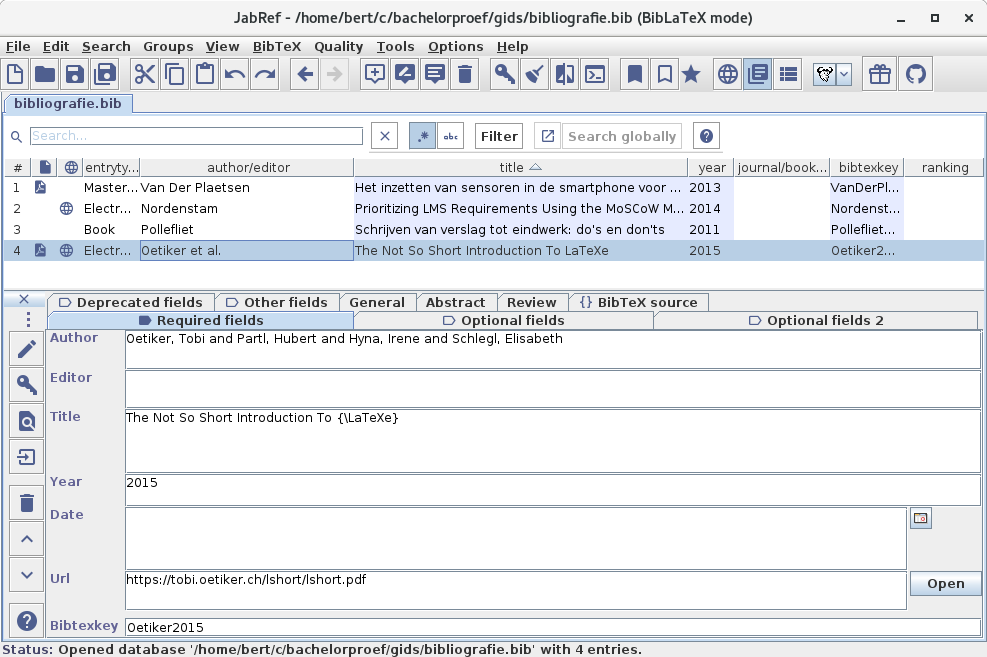
\includegraphics[width=\linewidth]{jabref-screenshot}
  \caption[JabRef]{\label{fig:jabref}\textbf{JabRef.} Centraal in de gebruikersinterface vind je een lijst van de verschillende bronnen in deze bibliografische databank. De pdf-icoontjes links bij de tweede en vierde bron geven aan dat de bron lokaal opgeslagen is als pdf. Als je hierop klikt, wordt de pdf geopend. De ketting-icoontjes die bij verschillende bronnen voorkomen duiden op een url die je in de webbrowser kan openen als je hierop klikt. Als je een bron selecteert, dan krijg je onderaan links invulvakken te zien met de bijgehouden metadata voor die bron. Deze worden opgedeeld in verschillende tabbladen, o.a.~verplichte gegevens (``Required fields''), optionele (``Optional'') en andere (``Other fields''), enz. In dit geval zijn de namen van de auteurs ingevuld (zie Sectie~\ref{sec:algemene_bibliografische_gegevens}). Er zijn in dit geval geen redacteurs (``Editors''), en dat veld is dan ook leeg gebleven. Het veld ``Citationkey'' onderaan is automatisch gegenereerd (zie Sectie~\ref{sub:jabref_instellingen}) door te klikken op de knop met het sleutelsymbool en label ``Generate'' rechts van het invulvak. Rechtsonder zie je een ``Preview,'' wat een idee zou moeten geven van hoe de referentie er uit zal zien in de bibliografie.}

\end{figure}

\subsection{JabRef instellingen}%
\label{sub:jabref_instellingen}

Wanneer je JabRef voor het eerst opent, is het nuttig om volgende instellingen aan te passen via Options > Preferences:

\begin{itemize}
  \item \textbf{General:} Default bibliography mode: wijzig dit naar biblatex. In de standaardinstelling (BibTeX) is er geen ondersteuning voor Unicode of voor de APA-stijl.
  \item \textbf{Entry preview:} Selecteer in de beschikbare stijlen de APA-stijl. Je krijgt dan rechtsonder in het venster een voorbeeld van de opmaak van de referentie in de APA-stijl. Dit is niet perfect, maar geeft wel een idee van hoe de bronvermelding er uit zal zien in de bibliografie.
  \item \textbf{Linked Files:} en geef een directory op voor het bijhouden van PDFs van de gevonden bronnen onder ``Main file directory''. Het is heel interessant om de gevonden artikels te downloaden en onder die directory bij te houden. Nog beter is om als naam van het bestand de BibTeX citation key te nemen (bv.\ Knuth1998.pdf). Je kan het bestand dan makkelijk openen vanuit JabRef.
\end{itemize}

Je kan de andere instellingen nakijken en eventueel naar wens aanpassen, maar de hierboven opgesomde zijn de belangrijkste.

\section{Een bibliografie invoegen in een {\LaTeX}-document}%
\label{sec:een_bibliografie_invoegen_in_een_latex_document}

Eens je enkele bronnen in een Bib{\LaTeX}-bestand hebt opgeslagen, kan je die gebruiken in je {\LaTeX}-document. In de {\LaTeX}-sjablonen voor het onderzoeksvoorstel en voor de bachelorproef zit de APA-stijl al ingebakken en je hoeft je dus helemaal geen zorgen te maken over de correcte opmaak. Dit gebeurt automatisch, mits je de bibliografische gegevens (bv.\ titel, auteur, jaar van publicatie) correct bijhoudt in Jabref.

Voor de volledigheid geven we hier de nodige instructies om dit ook in andere {\LaTeX}-documenten te kunnen toepassen.

Je hebt minstens een {\LaTeX}-bestand nodig en een Bib{\LaTeX}-bestand. In het {\LaTeX}-bestand moet je de in de ``preamble'' (d.w.z.\ vóór het \texttt{{\textbackslash}begin\{document\}} comman\-do) volgende instructies toevoegen:

\begin{minted}[frame=lines,linenos]{latex}
  \usepackage[backend=biber,style=apa]{biblatex}
  \DeclareLanguageMapping{dutch}{dutch-apa}
  \addbibresource{<naam van je BibLaTeX-bestand>.bib}
\end{minted}

De eerste regel zorgt er voor dat de APA-stijl wordt toegepast. De tweede regel zorgt er voor dat eventueel door {\LaTeX} gegenereerde tekst in het Nederlands wordt weergegeven. De derde regel zorgt er voor dat het opgegeven bibliografische databankbestand als bron kan gebruikt worden om referenties op te zoeken.

Achteraan het {\LaTeX}-bestand moet je dan de volgende instructie toevoegen:

\begin{minted}[frame=lines,linenos]{latex}
  \printbibliography
\end{minted}

Als je dit doet in een nieuw document en je compileert op dit punt, zal je wellicht merken dat er nog geen bibliografie wordt weergegeven. Dat komt omdat je nog geen referenties hebt toegevoegd. In een bibliografie mogen immers enkel werken vermeld worden waar ook effectief naar gerefereerd wordt in de tekst.

Over refereren kan je meer lezen in sectie~\ref{sec:bibliografie-refereren}.

\subsection{Wat als de bibliografie niet verschijnt?}%
\label{ssec:wat_als_de_bibliografie_niet_verschijnt}

Als je toch refereert in de tekst, maar je ziet na compileren nog steeds geen bibliografie, dan kan je volgende zaken controleren. Kijk ook naar de uitvoer van de compilatie voor foutboodschappen die je kunnen helpen bij het oplossen van het probleem.

\begin{itemize}
  \item Zijn er referenties in de tekst? \verb|\textcite| of \verb|\autocite| moet minstens één keer gebruikt worden.
  \item Misschien is bij het genereren van het PDF-document de bibliografie niet gecompileerd. In {\TeX}studio kan je dit forceren door in de menubalk te kiezen voor ``Tools > Bibliography'' (of sneltoets F8). Dan wordt \texttt{biber} uitgevoerd die alle referenties in de tekst opzoekt en het nodige doet om de bibliografie te genereren. Daarna moet je nog eens compileren (``Tools > Build \& View'' of F5) en nu zou de bibliografie moeten verschijnen.
  \item Als je in de PDF op de plaats van een referentie de ``citation key'' in het vet ziet staan, dan betekent het dat deze niet gevonden is in de bibliografische databank. Controleer of je de juiste citation key hebt gebruikt en of deze inderdaad voorkomt in het Bib{\LaTeX}-bestand.
\end{itemize} 

\section{Soorten bronnen}%
\label{sec:soorten_bronnen}

De bedoeling van een bibliografie is de lezer toelaten jouw bronnen zelf op te zoeken en te beoordelen op betrouwbaarheid. Dat betekent dat je voldoende informatie moet opgeven zodat de bron terug te vinden is. Afhankelijk van het soort bron moet je andere, specifieke informatie opgeven. Dit wordt verderop uitgediept.

Bij het toevoegen van een nieuwe bron aan een bibliografische databank moet je eerst het type selecteren (zie Afbeelding~\ref{fig:jabref-entrytypes}).

\begin{figure}
  \centering
  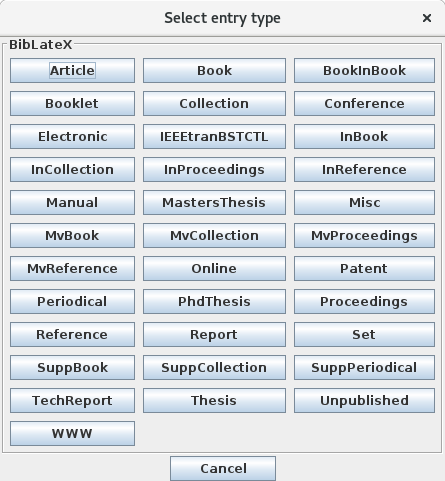
\includegraphics[width=0.6\linewidth]{img/jabref-entrytypes}
  \caption[Soorten bronnen in JabRef]{\label{fig:jabref-entrytypes}\textbf{Soorten bronnen in JabRef.} Bij het toevoegen van een nieuwe bron in JabRef (Ctrl+N) moet je eerst het soort publicatie kiezen. Afhankelijk van het soort moet in de literatuurlijst immers andere informatie gegeven worden.}
\end{figure}

Bib{\LaTeX} onderscheidt onder andere de volgende soorten bronnen:

\begin{description}
  \item[Article] Een artikel in een wetenschappelijke journal;
  \item[Online] Een online gevonden bron zoals blog-artikel van een vakexpert, video van een presentatie op een vakconferentie, artikel in een online publicatie zoals Dzone of InfoQ, enz. (synoniemen: WWW, Electronic);
  \item[Book, InBook] Een boek of hoofdstuk in een boek;
  \item[Thesis] Een scriptie of eindwerk van een student (bachelorproef, masterthesis, doctoraatsproefschrift);
  \item[Report] Een (onderzoeks-)rapport, typisch uitgegeven door een hoger onderwijsinstelling, onderzoeksgroep, overheidsinstelling, bedrijf, enz.
  \item[InProceedings] Een artikel in de ``proceedings'' van een conferentie, een boek waar\-in alle artikels gebundeld zijn die op de conferentie werden gepresenteerd;
  \item[enz.] Er zijn nog andere soorten bronnen, maar deze komen minder vaak voor of zijn niet relevant voor een bachelorproef informatica.
\end{description}

\section{Automatisch invullen van bibliografische gegevens}%
\label{sec:automatisch_invullen_van_bibliografische_gegevens}

Sommige tertiaire bronnen zoals ScienceDirect, Springer, Google Scholar, enz.\ bieden de mogelijkheid om de nodige informatie automatisch in te vullen. Dat kan op verschillende manieren.

Op de webpagina voor het gevonden artikel kan je de bibliografische gegevens in Bib{\LaTeX}-formaat kopiëren of downloaden. Zoek naar een link of knop met de vermelding ``Cite'', klik er op door en selecteer Bib{\LaTeX}. Kopieer de tekst en plak die in JabRef via het tabblad ``biblatex source''.

Een andere manier is via een unieke code die de bron identificeert. Voor boeken is dat het ISBN-nummer. Als je een nieuwe bron toevoegt (zie Figuur~\ref{fig:jabref-entrytypes}), kan je in het drop-down veld ``ID type'' ISBN kiezen en het nummer erin plakken. Klik vervolgens op ``Generate'' en de belangrijkste velden worden (in principe) meteen ingevuld.

Voor artikels die in journals gepubliceerd zijn, is er een gelijkaardig systeem: Ditigal Object Identifier of DOI. Dit is een unieke code die je kan vinden op de webpagina van het artikel. De vorm is meestal:

\begin{center}
  \texttt{https://doi.org/UITGEVER/ARTIKEL}

  bv. \texttt{https://doi.org/10.1016/j.ijinfomgt.2015.11.010}
\end{center}

Elke uitgever heeft een eigen code (bv. 10.1016 voor Elsevier, 10.1007 voor Springer, enz.) en binnen hun publicaties geven zij ook elk individueel artikel een ID. Bij het toevoegen van een nieuwe bron kies je als ``ID type'' voor DOI en kopieer en plak je het \texttt{UITGEVER/ARTIKEL}-gedeelte van de DOI-url (dus zonder \texttt{https://doi.org/}) in het invulveld.

Ook de documentatie over de TCP/IP-protocolstack kan je op deze manier toevoegen. Deze zijn online gepubliceerd\footnote{Zie \url{https://www.rfc-editor.org}} in de vorm van zgn.~RFC's (Request for Comment). Je kan als ``ID Type'' voor RFC kiezen en dan het nummer van de RFC invullen.

Merk op dat deze systemen niet altijd perfect werken, dus controleer altijd het resultaat! En misschien wil je nog informatie toevoegen die niet werd ingevuld via de ID, bv.\ de abstract, sleutelwoorden, enz.


\section{Algemene bibliografische gegevens}%
\label{sec:algemene_bibliografische_gegevens}

 Drie elementen zijn sowieso \emph{altijd} essentieel: de \textbf{auteur}, de \textbf{titel} van de bron en het \textbf{datum} (of tenminste het jaar) van publicatie. Als één van deze drie ontbreekt, wordt het bijzonder moeilijk om de oorsprong en de kwaliteit van de bron te evalueren. Dit soort bronnen kan je bijhouden ter info, maar zijn meestal niet geschikt om op te nemen in een bibliografie. Als de auteur onbekend is, is het immers niet mogelijk om te beoordelen of die wel de autoriteit heeft om op een objectieve en diepgaande manier over het onderwerp te schrijven. Als het jaartal niet opgegeven is, is het erg moeilijk om na te gaan in hoeverre deze bron nog niet achterhaald is door recentere ontwikkelingen in het vakgebied.

\subsection{Het Author-veld}%
\label{ssec:het_author_veld}

Enkele tips bij het invullen van auteursnamen:

\begin{itemize}
  \item Noteer de naam van auteurs in de vorm ``Familienaam, Voorna(a)m(en)''. Dus ``Van Vreckem, Bert'' en niet ``Bert Van Vreckem.'' In principe wordt de tweede notatie ook aanvaard, maar dit werkt enkel voor typische angelsaksische namen met een tweede voornaam (bv. ``Donald Ervin Knuth''). De eerste twee woorden worden beschouwd als voornamen, het laatste woord als de familienaam. ``Van'' wordt in dat geval dus verkeerdelijk beschouwd als tweede voornaam.
  \item Als de auteur een bedrijf of organisatie is, met een naam bestaande uit verschillende woorden, zet die dan tussen accolades: bv. ``\{The Linux Foundation\}''. Zoniet probeert {\LaTeX} dit als een persoonsnaam te interpreteren. ``Foundation'' wordt dan de familienaam, ``The'' en ``Linux'' de twee voornamen.
  \item Als je meerdere auteurs hebt, scheid elke naam dan met \texttt{and}, bv. ``Bernard, Anita and Buysse, Jens and Van Vreckem, Bert''.
  \item Na invullen van de auteursna(a)m(en) klik je op de knop met het sleutel-icoon (zie Figuur~\ref{fig:jabref}) om een unieke sleutel te genereren voor deze bron.
  \item Naast een auteurveld is er ook een veld voor eventuele redacteur(s) (\emph{editor}) voorzien. Minstens één van beide moet ingevuld zijn, soms allebei. Dit gebeurt bijvoorbeeld in een boek dat samengesteld is uit hoofdstukken die telkens door andere auteurs geschreven zijn en waar je naar één bepaald hoofdstuk wil verwijzen. Verderop vind je daar een voorbeeld van.
\end{itemize}

\subsection{Het Date-veld}%
\label{ssec:het_date_veld}

Data worden in Bib{\LaTeX} altijd in het formaat \texttt{jjjj-mm-dd} ingegeven (volgens de ISO-8601 standaard), dus eerst het jaar, dan de maand en tenslotte de dag, gescheiden met koppeltekens (-).

Als je de maand of de dag niet kent, vernoem je enkel het jaar.

Bij het importeren van bibliografische gegevens wordt soms niet het Date-veld ingevuld, maar Year. Dit is een overblijfsel van de Bib{\TeX} standaard, waar er aparte velden voorzien waren voor het jaartal (Year) en maand (Month, weergegeven door de eerste drie letters van de maand in het Engels: Jan, Feb, Mar, enz.).

Je kan de inhoud van het Year-veld (en desgevallend Month) het best naar Date kopiëren.

\subsection{Extra informatie bijhouden}%
\label{ssec:extra_informatie_bijhouden}

Probeer telkens zoveel mogelijk informatie bij te houden over je bronnen, zodat het later makkelijker wordt die terug te vinden. Dit is een tijdrovend proces, en niet al deze informatie wordt ook in de bibliografie opgenomen. Het raadplegen van de databank wordt wel een stuk makkelijker.

Enkele velden die zinvol zijn om altijd trachten in te vullen, ook al zijn ze niet verplicht en worden ze ook niet altijd in de bibliografie getoond:

\begin{description}
  \item[Abstract] Samenvatting van het artikel. Dit is meestal de eerste paragraaf van een artikel en wordt altijd duidelijk aangegeven.
  \item[DOI] of ``Digital Object Identifier''. Dit is een unieke code voor artikels in wetenschappelijke publicaties die het opzoeken makkelijker maakt (op voorwaarde dat de DOI gegeven is).
  \item[File] Naam van het bestand met het gedownloade artikel. Je kan vanuit JabRef het artikel openen in een PDF-viewer of desgevallend tekstverwerker.
  \item[Keywords] Kernwoorden i.v.m~het onderwerp, gescheiden door komma's.
  \item[Review] Je eigen opmerkingen over deze bron. Waarom heb je deze bijgehouden? Wat is het interessantste dat je er uit geleerd hebt?
  \item[URL] De URL waar je het artikel gevonden hebt. Deze URL wordt niet altijd in de bibliografie opgenomen, maar is altijd nuttig om bij te houden. Je kan vanuit JabRef de website openen in een webbrowser.
  \item[Urldate] de datum waarop je deze bron het laatst hebt geraadpleegd.
\end{description}

Let er tenslotte ook op dat je in Jabref \textbf{nooit speciale lettertekens gebruikt} die voor {\LaTeX} een specifieke betekenis hebben. Het gaat hier dan onder andere over het percentteken (\%), het hekje (\#), het dollarteken (\$), het ampersand-teken (\&) en de accolades (\{ en \}). Als je deze toch nodig hebt, moet je er meestal een backslash voor zetten, bv. ``\textbackslash\%'' of het geschikte commando voor dat specifieke teken gebruiken. Als je dit over het hoofd ziet, zal je compilatie mislukken en jammer genoeg is de foutboodschap vaak niet erg duidelijk.

\section{Specifieke bibliografische gegevens}%
\label{sec:specifieke_bibliografische_gegevens}

In deze sectie wordt voor de meest relevante soorten bronnen uitgelegd hoe deze correct bij te houden en in de bibliografie op te nemen. JabRef geeft zelf al enige aanwijzingen over welke informatie minstens nodig is: in het detailvenster (zie Afbeelding~\ref{fig:jabref}) moet je minstens het tabblad ``Required fields'' invullen. Voor elk soort publicatie (zie Sectie~\ref{sub:publicatievormen}) vind je verderop een overzicht van de in te vullen velden en wat die precies betekenen, en hoe de referentie in de literatuurlijst er uit zal zien.

\subsection{Article}%
\label{ssec:article}

Dit soort bron wordt enkel gebruikt voor artikels die verschenen zijn in een wetenschappelijke journal. Artikels in (vak)tijdschriften of kranten vallen hier \emph{niet} onder, maar daarvoor gebruik je het type Periodical.

Verplichte velden voor Article:

\begin{description}
  \item[Author] De naam van de auteur;
  \item[Title] De titel van het artikel;
  \item[Journaltitle] De naam van het tijdschrift;
  \item[Date] Verschijningsdatum (of -jaar) van het artikel;
  \item[Volume] De jaargang van het tijdschrift waarin het artikel verschenen is;
  \item[Number] Het nummer (binnen de jaargang) waarin het artikel verschenen is (soms niet gegeven);
  \item[Pages] Paginanummers
\end{description}

Voorbeeld broncode:
\begin{minted}[frame=lines,linenos,breaklines]{bibtex}
@Article{SabiEtAl2016,
  author       = {Sabi, Humphrey M. and Uzoka, Faith-Michael E. and Langmia, Kehbuma and Njeh, Felix M.},
  title        = {Conceptualizing a model for adoption of cloud computing in education},
  journaltitle = {International Journal of Information Management},
  date         = {2016},
  volume       = {36},
  number       = {2},
  pages        = {183--191},
  doi          = {10.1016/j.ijinfomgt.2015.11.010},
  url          = {http://www.sciencedirect.com/[...]8401215001115},
  abstract     = {Cloud computing is a pervasive computing [...]},
  keywords     = {Cloud computing, Educational technologies, [...]},
}
\end{minted}

In de bibliografie ziet dit er zo uit: \fullcitebib{SabiEtAl2016}

\subsection{Online}%
\label{ssec:online}

Onder dit type publicatie vallen vrijwel alle online bronnen die niet onder een andere categorie te plaatsen zijn: blogartikels, artikels in online vaktijdschriften of portaalsites, Youtube-video's van presentaties op vakconferenties, online documentatie, enz.

Merk op dat je de algemene website van organisaties, softwarepakketten, enz. \emph{niet} in je literatuurlijst mag opnemen. Deze kan je wel in een voetnoot zetten.

Deze velden moet je verplicht invullen:

\begin{description}
  \item[Author] Auteur(s) van de bron, spreker (in het geval van een video van een lezing op een conferentie), \ldots
  \item[Title] Titel van de bron, lezing, \ldots
  \item[Date] Datum (of jaar) van publicatie,
  \item[URL] naar de website waar de bron kan teruggevonden worden,
  \item[Urldate] Datum van laatste raadplegen,
\end{description}

Bij dit soort bronnen worden veel fouten gemaakt bij het refereren. Het is essentieel dat de URL wordt meegegeven en ook de datum van raadplegen. Het web is voortdurend in beweging, en het is mogelijk dat de inhoud van een webpagina in de loop van de tijd verandert (bv.\ fouten die verbeterd worden) of zelfs dat een website herstructureert en de URL dus op een gegeven manier niet meer geldig is. Door de datum van raadplegen op te geven, bied je de lezer nog de kans om terug te vinden hoe die website er op dat moment in de tijd uitzag, via bijvoorbeeld de Wayback Machine van het Internet Archive\footnote{\url{https://archive.org/web/}}.

Vergeet niet om de URL goed na te kijken en overbodige informatie te verwijderen, zoals:

\begin{itemize}
  \item \texttt{\&utm\_source=\ldots}, parameters in de URL die gebruikt worden om de herkomst van de bezoeker te traceren. Deze zijn niet nodig om de pagina terug te vinden.
  \item \texttt{\#:\textasciitilde:text=Highlighted\%20text}, code die bepaalde tekst op de pagina markeert.
\end{itemize}

Voorbeeld van een blogartikel:

\begin{minted}[frame=lines,linenos,breaklines]{bibtex}
@Online{LewisFowler2014,
  author    = {Lewis, James and Fowler, Martin},
  title     = {Microservices: a definition of this new architectural term},
  date      = {2014-03-25},
  url       = {http://martinfowler.com/articles/microservices.html},
  urldate   = {2016-09-01},
  abstract  = {The term "Microservice Architecture" has [...]},
  keywords  = {application architecture, web services, microservices},
}
\end{minted}

In de bibliografie wordt dit: \fullcitebib{LewisFowler2014}

Een ander voorbeeld, deze keer van een presentatie op een vakconferentie die op Youtube is gepubliceerd. Omdat er niet meteen een apart veld voorzien is voor het vermelden van de naam van de conferentie, is die hier in het titelveld verwerkt.

\begin{minted}[frame=lines,linenos,breaklines]{bibtex}
@Online{Hykes2013,
  author       = {Solomon Hykes},
  title        = {The future of Linux Containers (PyCon 2013)},
  date         = {2013-03-21},
  url          = {https://www.youtube.com/watch?v=wW9CAH9nSLs},
  urldate      = {2016-09-01},
  abstract     = {At PyCon Solomon Hykes shows docker to the public for the first time.},
}
\end{minted}

In de bibliografie: \fullcitebib{Hykes2013}

\subsection{Book}%
\label{ssec:book}

Dit type gebruik je voor (e-)boeken die ``officieel'' uitgegeven zijn en dus een ISBN-nummer hebben.

Minstens volgende velden moeten dan ingevuld zijn:

\begin{description}
  \item[Author] De auteur(s) van het boek,
  \item[Date] Jaartal waarin het boek werd uitgegeven,
  \item[Title] Titel van het boek,
  \item[Publisher] Naam van de uitgeverij.
\end{description}

Optioneel kan je ook volgende informatie aanvullen:

\begin{description}
  \item[Subtitle] ondertitel van het boek,
  \item[Edition] Nummer van de uitgave of druk,
  \item[Location] Stad waar de uitgeverij gevestigd is,
  \item[ISBN] Het ISBN-nummer van het boek (ter info, wordt nooit getoond in de bibliografie),
  \item[URL] Naar de pagina over het boek op de website van de uitgeverij. \textbf{Let op!} Dit is \emph{niet} de URL van een webshop waar je het boek kan kopen, noch een link naar Google Books en zeker niet naar een illegale downloadsite!
\end{description}

Voorbeeld:
\begin{minted}[frame=lines,linenos,breaklines]{bibtex}
@Book{Aitchison2011,
  author    = {Aitchison, Ron},
  date      = {2011},
  title     = {Pro DNS and BIND 10},
  isbn      = {9781430230489},
  publisher = {Apress},
}
\end{minted}

In de bibliografie:
\fullcitebib{Aitchison2011}

\subsection{InBook}%
\label{ssec:inbook}

Dit type gebruik je als je wil verwijzen naar een specifiek hoofdstuk in een boek. Minstens volgende velden moeten dan ingevuld zijn:

\begin{description}
  \item[Author] De auteur(s) van het hoofdstuk,
  \item[Editor] De redacteur(s) van het boek (indien van toepassing),
  \item[Date] Jaartal waarin het boek werd uitgegeven,
  \item[Title] Titel van het \emph{hoofdstuk},
  \item[Pages] Begin- en eindpagina van het hoofdstuk,
  \item[Booktitle] Titel van het \emph{boek},
  \item[Publisher] Naam van de uitgeverij.
\end{description}

Optioneel kan je ook volgende informatie aanvullen:

\begin{description}
  \item[Subtitle of Booksubtitle] ondertitel van het hoofdstuk of boek, resp.,
  \item[Edition] Nummer van de uitgave of druk,
  \item[Location] Stad waar de uitgeverij gevestigd is,
  \item[ISBN] Het ISBN-nummer van het boek (ter info, wordt nooit getoond in de bibliografie).
\end{description}

Bij een boek is het ongebruikelijk om een URL op te geven. Als je bijvoorbeeld ter info voor jezelf de URL van het boek op de website van de uitgever wil bijhouden, doe je dit best in een ander veld, bv. Comment of Review.

Voorbeeld
\begin{minted}[frame=lines,linenos,breaklines]{bibtex}
@InBook{Meyr2008,
  author       = {Meyr, Herbert},
  title        = {Forecast Methods},
  booktitle    = {Supply Chain Management and Advanced Planning},
  date         = {2008},
  editor       = {Stadtler, Hartmut and Kilger, Christoph},
  booksubtitle = {Concepts, Models, Software, and Case Studies},
  edition      = {4e editie},
  publisher    = {Springer},
  location     = {Heidelberg},
  isbn         = {978-3-540-24814-9},
  pages        = {461--472},
  comment      = {https://www.springer.com/us/book/9783540248149},
}
\end{minted}

In de bibliografie ziet dit er zo uit:
\fullcitebib{Meyr2008}

\subsection{Thesis}%
\label{ssec:thesis}

Onder dit type publicatie vallen doctoraatsproefschriften, masterthesissen en bachelorproeven. Dit zijn de in te vullen velden:

\begin{description}
  \item[Author] De auteur van de thesis (student of doctorandus),
  \item[Title] Titel van de scriptie
  \item[Date] Jaar of datum van indienen
  \item[Type] Soort scriptie: Bachelorproef, masterthesis, doctoraatsthesis, \ldots
  \item[Institution] Naam van de hogeschool of universiteit waar de thesis werd ingediend
\end{description}

Voorbeeld:
\begin{minted}[frame=lines,linenos,breaklines]{bibtex}
  @Thesis{VanDerPlaetsen2013,
  author      = {Van Der Plaetsen, Thomas},
  date        = {2013},
  institution = {Hogeschool Gent},
  title       = {Het inzetten van sensoren in de smartphone voor het
                 verbeteren van de fanbeleving},
  type        = {Bachelorproef},
}
\end{minted}

Resultaat in de bibliografie:
\fullcitebib{VanDerPlaetsen2013}

\subsection{Report}%
\label{ssec:report}

Onder Report vallen onderzoeksrapporten uitgegeven door onderzoeksgroepen van universiteiten of hogescholen, overheidsinstellingen of bedrijven.

Verplichte velden:

\begin{description}
  \item[Author] De auteur(s)
  \item[Date] Datum of jaar van publicatie
  \item[Title] Titel van het onderzoeksrapport
  \item[Type] Het soort rapport. In JabRef is er een dropdown-menu met de meest voorkomende types. Meestal vul je hier \texttt{resreport} in, de afkorting van ``research report''.
  \item[Institution] Instelling die het rapport uitgegeven heeft
\end{description}

Optionele velden:

\begin{description}
  \item[Subtitle] Ondertitel van het rapport
  \item[URL] URL waar de instelling het rapport gepubliceerd heeft
  \item[Urldate] Datum waarop je het rapport geraadpleegd hebt
\end{description}

Voorbeeld:
\begin{minted}[frame=lines,linenos,breaklines]{bibtex}
@Report{DeMarez2022,
  author      = {De Marez, Lieven and Sevenhant, Robbe and ...},
  date        = {2022},
  institution = {imec},
  title       = {imec.digimeter 2022},
  type        = {resreport},
  subtitle    = {Digitale trends in Vlaanderen},
  url         = {https://www.imec.be/nl/...},
  urldate     = {2023-05-01},
}
\end{minted}

Resultaat in de bibliografie:
\fullcitebib{DeMarez2022}

\subsection{InProceedings}%
\label{ssec:inproceedings}

Dit soort bron wordt gebruikt voor artikels die gepubliceerd zijn in het verslag (proceedings) van een \emph{wetenschappelijke} conferentie. Verplichte velden:

\begin{description}
  \item[Author] Naam van de auteur(s),
  \item[Title] Titel van het artikel,
  \item[Booktitle] De naam van de conferentie,
  \item[Date] Datum (of jaar) waarin de conferentie doorging.
\end{description}

Daarnaast kan je optioneel ook volgende velden invullen:

\begin{description}
  \item[URL] naar de website van de conferentie waar het artikel kan gevonden (eventueel rechtstreeks naar de pdf);
  \item[Urldate] datum waarop je deze bron het laatst geraadpleegd hebt.
  \item[DOI] op voorwaarde dat er één toegewezen is aan dit artikel.
\end{description}

Voorbeeld:
\begin{minted}[frame=lines,linenos,breaklines]{bibtex}
@InProceedings{VanVreckemEtAl2013,
  author    = {Van Vreckem, Bert and Borodin, Dmitriy and De Bruyn, Wim and Now\'{e}, Ann},
  title     = {A Reinforcement Learning Approach to Solving Hybrid Flexible Flowline Scheduling Problems},
  booktitle = {Multidisciplinary International Scheduling Conference (MISTA) 2013},
  date      = {2013},
  url       = {https://expertise.hogent.be/files/.../hffsp_la.pdf},
  urldate   = {2016-09-01},
  abstract  = {In this paper, we present a method based on Learning Automata to solve Hybrid Flexible Flowline Scheduling  Problems [...].},
}
\end{minted}

In de bibliografie ziet dit er zo uit: \fullcitebib{VanVreckemEtAl2013}

\subsection{Andere}%
\label{ssec:andere}

In JabRef zijn nog andere soorten bronnen gedefinieerd, maar deze zijn minder relevant voor een eindwerk of paper (bv. Legislation, Patent, \ldots) of komen overeen met een van de hierboven opgesomde types.

Electronic en WWW zijn bijvoorbeeld synoniemen voor Online.

Handleidingen vallen onder het type Manual, dat je kan invullen volgens de regels van een Book (als deze in boekvorm uitgegeven is), of als een Online bron (als deze online beschikbaar is).

\section{Refereren in de tekst}%
\label{sec:bibliografie-refereren}

Als je na het opvullen van je bibliografische databank met bronnen het {\LaTeX}-do\-cu\-ment zou compileren, zal je waarschijnlijk merken dat al deze nieuwe bronnen niet zichtbaar zijn in de bibliografie. Dit komt omdat in een bibliografie \textbf{enkel werken mogen opgenomen zijn waarnaar verwezen wordt vanuit de tekst}. {\LaTeX} doet dit standaard automatisch, dus als je bronnen in de lijst mist, dan betekent dit dat je die niet in de tekst gebruikt hebt.

Voor het refereren naar bronnen in de tekst zijn er twee commando's gangbaar: \texttt{{\textbackslash}textcite} en \texttt{{\textbackslash}autocite}. Het eerste commando geeft een narratieve referentie, het tweede commando geeft een referentie tussen haakjes. Het is gebruikelijk om het eerste commando te gebruiken als je de naam van de auteur(s) in de tekst vermeldt, en het tweede commando als je de naam van de auteur(s) niet in de tekst vermeldt.

\subsection{Narratieve referenties}%
\label{ssec:narratieve_referenties}

Een voorbeeld van een narratieve referentie:

\begin{verbatim}
An overview is provided in the survey by~\textcite{RibasEtAl2010}.
For a real-life case-study of applying genetic algorithm ``on top''
of a Mixed Integer Linear Programming model, we refer
to~\textcite{BorodinEtAl2011}.
\end{verbatim}

wat resulteert in:

\begin{quotation}
  An overview is provided in the survey by Ribas, et al. (2010). For a real-life case-study of applying genetic algorithm ``on top'' of a Mixed Integer Linear Programming model, we refer to Borodin, et al. (2011).
\end{quotation}

\subsection{Referenties tussen haakjes}%
\label{ssec:referenties_tussen_haakjes}

Referenties tussen haakjes gebruik je als je de naam van de auteur(s) niet in de tekst vermeldt, bijvoorbeeld als je vakterm definieert, bij een letterlijk citaat of parafrasering of in het bijschrift van een figuur die je overgenomen hebt uit een bron.

\begin{verbatim}
Reinforcement Learning (RL) is a technique that allows an agent
to learn how to maximize a numerical reward
signal~\autocite{SuttonBarto1998}.
\end{verbatim}

wat resulteert in:

\begin{quotation}
  Reinforcement Learning (RL) is a technique that allows an agent to learn how to maximize a numerical reward signal (Sutton \& Barto, 1998).
\end{quotation}

\section{Controle}%
\label{sec:bibliografie-controle}

Het is belangrijk om na het genereren van de PDF met je finale paper of eindwerk nog eens goed te controleren of de referenties en bibliografie correct opgemaakt zijn.

\begin{itemize}
  \item Zijn de namen van de auteurs correct weergegeven? Indien de auteur een bedrijf of organisatie is, is de naam volledig weergegeven of geïnterpreteerd als een persoonsnaam?
  \item Controleer dat er geen titels VOLLEDIG IN HOOFDLETTERS staan en zet deze zo nodig om.
  \item Is er een minstens een jaartal opgegeven? Controleer ook dat nergens nog het Year- of Mont-veld ingevuld is en dat de inhoud naar Date verhuisd is.
  \item Zijn de URLs correct weergegeven? Zijn er geen parameters of tracking codes in de URL geslopen?
  \item Hebben Online-bronnen ook een datum van raadplegen?
  \end{itemize}

\section{Samenvatting}%
\label{sec:bibliografie-samenvatting}

Het bijhouden van al je bronnen is tijdrovend, maar essentieel voor een goed onderbouwde bachelorproef! Besteed hier dus de nodige aandacht aan.

\begin{itemize}
  \item Zet je bibliografische databank op (bv.\ met JabRef) voordat je op zoek gaat naar informatie over je onderwerp en hou van wat je vindt nauwgezet zoveel mogelijk informatie bij.
  \item Zorg dat je altijd minstens de auteur, titel en jaartal hebt en daarnaast minstens alle andere verplichte informatie voor dat type publicatie correct noteert.
  \item Selecteer het correcte type publicatie en zorg dat in elk geval de verplichte gegevens telkens ingevuld zijn.
  \item Vergeet niet het resultaat te controleren en zo nodig aan te passen.
\end{itemize}

\chapter{Onderzoeksmethoden}
\label{ch:onderzoeksmethoden}

In dit onderwerp vind je aanbevelingen in verband met een aantal vaak gebruikte onderzoeksmethoden. Meer bepaald bespreken we de aanpak van een vergelijkende studie, hoe je correct experimenten opzet en hoe je op een correcte manier rapporteert over bekomen resultaten (in het bijzonder cijfermateriaal).

% Belang van correcte methodologie
%
% Voorbeelden:
% - enquêtes (verwijzen naar Saunders?)
%     - pitfalls: respons, slechte vragen, slechte verwerking, te laat opgengesteld
%     - onderzoekskader, steekproefmethode (benader aselecte steekproef)
%     - stel vragen zo dat je op zoek kan gaan naar verbanden!
%     - tip: neem deel aan enquêtes, bv. van iMinds => voeling met vraagstelling
% - interviews (kwalitatief)
%     - wanneer? Casus leren kennen, vakexpert, requirements-analyse
%     - Goed voorbereiden, opnemen, transcriptie uitschrijven, verwerken
% - experiment
% - vergelijkende studie
% - casus/case study
% - doorlichting beveiliging: risico-analyse Chris Jackson, Network Security Auditing. Cisco Press. 2010.
%
% wanneer pas je elk toe?
% Vaak heb je een combinatie van deze technieken nodig om je onderzoeksvra(a)g(en) goed en onderbouwd te kunnen beantwoorden.

\section{De vergelijkende studie}
\label{sec:vergelijkende-studie}

Een type onderwerp dat vaak gekozen wordt voor een bachelorproef is een vergelijkende studie. Je bent op zoek naar een oplossing voor een probleem in de vorm van een software- of hardware-product, platform, dienst, enz. De bedoeling van de studie is om alle mogelijke alternatieven naast elkaar te zetten en een keuze te maken over de meest geschikte.

De ervaring leert dat een vergelijkende studie pas echt goed is als er een concreet doel is, een reële situatie waar de geselecteerde oplossing ook werkelijk zal toegepast worden. Het gevaar bestaat dat de studie zich beperkt tot het achter elkaar opsommen van enkele arbitrair gekozen mogelijkheden. Er volgt een paragraafje uitleg, soms gewoon van Wikipedia gehaald, met een opsomming van wat voor- en nadelen, maar niet gestructureerd en zonder rode draad. Een bepaald aspect als ``gebruiksvriendelijkheid'' wordt dan bijvoorbeeld in één product besproken, maar niet voor de andere, enz. De eigen inbreng is dan miniem: een dagje zoeken op Wikipedia, samenvatten of verder uitschrijven, klaar. Dit is op zich dus onvoldoende.

Maar hoe pak je het dan \emph{wel} aan?

Laat ons veronderstellen dat je na je afstuderen aan de slag wil als webontwikkelaar, en je bent op zoek naar een geschikt PHP-framework om je websites mee te bouwen.

\subsection{Requirements-analyse}
\label{ssec:requirements-analyse}

Om een goede keuze te maken begin je met het verzamelen van \emph{requirements}, zowel \textit{functionele} als \emph{niet-functionele}, bijvoorbeeld:

\begin{itemize}
\item Functionele requirements
  \begin{itemize}
  \item Ondersteuning voor HTML5/CSS3
  \item Responsive design
  \item Er moet een authenticatiemodule in zitten dat OpenID, Facebook- en Google-authenticatie ondersteunt
  \item \ldots
  \end{itemize}
\item Niet-functionele requirements
  \begin{itemize}
  \item Moet bestand zijn tegen de top-10 beveiligingsproblemen van OWASP\footnote{\url{https://www.owasp.org/index.php/Category:OWASP_Top_Ten_Project}}
  \item Wachtwoorden worden opgeslagen volgens de state-of-the art (\emph{salted} en \emph{hashed})
  \item Moet open source zijn
  \item Moet gratis zijn
  \item \ldots
  \end{itemize}
\end{itemize}

Als je het onderzoek doet voor een ``klant'' (i.e. je co-promotor), dan betrek je uiteraard alle belanghebbenden bij dit proces! Je lijst de requirements op en verdeelt ze onder naar belangrijkheid, bijvoorbeeld via de MoSCoW-techniek~\parencite{Nordenstam2014}. Je verdeelt de requirements dan in categorieën zoals ``must-have'', ``should-have'' en ``nice-to-have''.

\subsection{Long list}
\label{ssec:long-list}

Dan zoek je \emph{zoveel mogelijk} alternatieven die in aanmerking komen om gebruikt te worden, m.a.w.~al diegenen die je kan vinden. Je noemt ze in deze \emph{long list} (die soms kan bestaan uit tientallen alternatieven) bij naam, met eventueel vermelding van een website en een beschrijving in één zin. Elk alternatief toets je af aan de requirements, voor zover dit al mogelijk is aan de hand van informatie die je op de website vindt of via andere bronnen. Zaken die je niet kan verifiëren laat je gewoon open om later na te kijken of misschien zelfs te negeren (als het bv.~gaat om een onbelangrijke feature, of als verschillende andere must-haves niet voldaan zijn). Je sorteert de long list dan volgens het aantal voldane requirements, en maakt hier een overzichtelijke tabel van. Hopelijk heb je een aantal alternatieven overgehouden die voldoen aan alle must-haves en zoveel mogelijk should-haves en nice-to-haves.

\subsection{Short list en proof-of-concept}
\label{ssec:short-list-poc}

 De meest veelbelovende alternatieven weerhoud je voor de volgende fase. De alternatieven in deze \emph{short list} ga je in meer detail bespreken en verder tegenover elkaar afwegen. Zet eventueel een \emph{proof-of-concept} op (zie Sectie \ref{sec:poc-testopstelling}), waarin je één of enkele van de meest veelbelovende alternatieven uitprobeert aan de hand van eenzelfde vastgelegd \emph{scenario} waarin je de requirements die je nog niet hebt kunnen verifiëren aan bod laat komen.

\subsection{Conclusie}
\label{ssec:vgl-studie-conclusie}

Tenslotte geef je je \emph{aanbeveling}, het alternatief dat het beste aansluit bij de requirements, en wat eventueel nog moet gedaan worden om het nog beter geschikt te maken.

\section{Proof-of-concept of testopstelling}
\label{sec:poc-testopstelling}

Met een proof-of-concept of testopstelling wil je aantonen dat een voorgestelde of veelbelovende oplossing voor de onderzoeksvraag ook realiseerbaar is in de praktijk. Vaak is het nodig verschillende varianten naast elkaar op te zetten, zodat je nog onderling kan vergelijken.

Een goede testopstelling voldoet aan drie eigenschappen \autocite{Liberman2015}:

\begin{description}
  \item[Reproduceerbaarheid] in staat zijn om de testopstelling opnieuw op te zetten (eventueel door een onafhankelijke partij) en de analyse opnieuw uit te voeren zodat je kan verifiëren dat je gelijkaardige resultaten krijgt.
  \item[Repliceerbaarheid] lijkt op het voorgaande, maar is sterker uitgedrukt: bij een repliceerbare testopstelling is het mogelijk dat een onafhankelijke partij deze \textit{exact} opnieuw kan opzetten en dezelfde resultaten zal bekomen.
  \item[Herbruikbaarheid] varianten kunnen opzetten van de testomgeving zodat deze onderling kunnen vergeleken worden.
\end{description}

De beste manier om dit te bereiken is door het proces te automatiseren.

\subsection{Reproduceerbaarheid}
\label{ssec:reproduceerbaarheid}

Een minimumverwachting van de tekst van een bachelorproef is dat de lezer in staat moet zijn om aan de hand van de beschrijving de testopstelling te reproduceren en je conclusies moet kunnen verifiëren. Dat betekent ook dat je beschrijving voldoende gedetailleerd moet zijn. Geef aan het begin van deze sectie in je tekst een duidelijke afbeelding met een schema van de opgezette testomgeving. Beschrijf vervolgens in detail:

\begin{itemize}
  \item Welke hardware werd er gebruikt? Computers, netwerkapparatuur, andere ict-infrastructuur. Welke specificaties hebben deze apparaten (CPU, geheugen, type en grootte harde schijven, snelheid netwerkinterfaces, enz.)?
  \item Welke softwarepakketten zijn er geïnstalleerd die relevant zijn voor de testopstelling? Welke specifieke edities en/of versienummers?
  \item Hoe is de installatieprocedure precies verlopen? Welke instellingen zijn er aangepast, en hoe zijn alle componenten geconfigureerd?
\end{itemize}

\subsection{Repliceerbaarheid}
\label{ssec:repliceerbaarheid}

Het is zowel voor jezelf als voor de lezer van je bachelorproef belangrijk om het opzetten van de testomgeving zo veel mogelijk te automatiseren, bijvoorbeeld door het schrijven van een installatiescript. Op deze manier bereik je de \textit{repliceerbaarheid} van je testopstelling.

Voor veel situaties kan je een proof-of-concept uitwerken met virtuele machines. Op die manier creëer je een afgeschermde omgeving zonder dat je extra software moet installeren op je fysieke systeem. Vagrant\footnote{\url{https://www.vagrantup.com/}} is een interessante tool om reproduceerbare virtuele testomgevingen volledig geautomatiseerd op te zetten. Het is zelf geen virtualisatiesysteem, maar het spreekt VirtualBox, VMWare of Hyper-V aan vanop de command-line. Je beschrijft in een configuratiebestand (\texttt{Vagrantfile}) welke VMs je nodig hebt, met hoeveel processorkernen/geheugen/schijfruimte, met welk besturingssysteem, enz. Via een script of configuration management system (zoals Ansible) kan je de precieze configuratie van de VMs beschrijven (installatie software, gebruikers, netwerkservices, configuratiebestanden, enz.). De code/configuratie om een Va\-grant-\-omgeving op te zetten is erg compact, volledig tekstgebaseerd en kan dus worden bijgehouden in een versiebeheersysteem.

Ook Docker\footnote{\url{https://docker.com/}} is een interessante tool hiervoor. Docker is een vorm van zgn.~containervirtualisatie. Virtuele machines (containers) hebben geen eigen OS, maar bevatten in principe enkel een applicatie. Het OS van het fysieke systeem wordt hergebruikt door de containers. Dat maakt dat containers een stuk efficiënter zijn qua schijf- en geheugengebruik voor het fysieke systeem. Er zijn echter een aantal beperkingen waardoor Docker niet altijd bruikbaar is als platform voor een testopstelling.

Als je merkt dat je een fout gemaakt hebt in de configuratie van je testopstelling, dan kan je het installatiescript aanpassen en de gehele testomgeving opnieuw opzetten. Als je dit manueel zou moeten doen, ben je wellicht minstens een dag kwijt. Bovendien heb je de kans dat je een kleinigheid over het hoofd ziet en dus niet in staat bent de testomgeving opnieuw exact te replicerne. Het initialiseren van een Linux-VM met Vagrant of Docker duurt typisch slechts enkele minuten. Windows-systemen nemen een stuk meer tijd in beslag. Het OS is op zich al een stuk groter\footnote{Ca.~4GB voor Windows Server Core tegenover 256 à 512MB voor een minimale installatie van een Linux distributie. Installatie van applicaties hebben nog een bijkomende impact op de schijfgrootte van de VM.}

Een uitgebreide handleiding van Vagrant of Docker valt buiten het bereik van deze gids. Een voorbeeld ter illustratie is te vinden op \url{https://github.com/bertvv/lampstack}. Hier wordt een Apache webserver opgezet met een MariaDB databank, PHPMyAdmin, en Wordpress.

\subsection{Herbruikbaarheid}
\label{ssec:herbruikbaarheid}

Door het gehele proces te automatiseren creëer je een bijkomend voordeel: het is een stuk makkelijker om gelijkaardige varianten van een testopstelling te creëren. Stel dat je de performantie-impact van een cache op een databasesysteem wil meten. De installatie van beide varianten (met/zonder cache) zijn zeer gelijkaardig. In een Vagant-omgeving kan je 2 VMs creëren, met hetzelfde installatiescript voor de basisopstelling, en een apart script om de verschillende configuratie-varianten te realiseren.

\section{Experimenten uitvoeren en verzamelen van kwantitatieve data}
\label{sec:experimenten-uitvoeren}

Wanneer je een experiment opzet waarbij je kwantitatieve data gaat verzamelen, bijvoorbeeld voor een performantievergelijking, gelden dezelfde richtlijnen als bij een proof-of-concept: het is belangrijk dat die reproduceerbaar, repliceerbaar en herbruikbaar is. Wellicht start je vanaf een vooraf gedefinieerde testopstelling, en ga je herhaaldelijk eenzelfde handeling uitvoeren en metingen doen.

Ook hier is het belangrijk het uitvoeren van het experiment en het opslaan van testresultaten te automatiseren, bijvoorbeeld aan de hand van een shell-script. Als je een experiment manueel moet uitvoeren, wordt dit al snel een erg tijdrovende bezigheid. Stel je voor dat je telkens je het experiment wil uitvoeren op een knop moet drukken, ongeveer vijf à tien minuten moet wachten en dan de uitvoer naar Excel moet kopiëren en plakken en dan het rekenblad nog eens moet bewerken zodat je enkel de cijfers overhoudt om statistisch te verwerken. Deze werkwijze is onhoudbaar. Je moet immers voortdurend aanwezig en aandachtig blijven tijdens het uitvoeren. Bij elke manuele handeling is er bovendien een kans op het maken van fouten.

Een script dat het experiment in verschillende varianten kan uitvoeren zonder interactie door de gebruiker, en ook meteen de resultaten kan opslaan in een geschikt bestandsformaat bespaart je enorm veel tijd. Je kan het experiment 's nachts laten draaien en op die manier kan je het ook voldoende herhalen om statistisch bruikbare resultaten te bekomen. Als een experiment mislukt, volstaat het om het script te verbeteren en het opnieuw uit te voeren. Het is ook makkelijker om verschillende varianten te schrijven (zoals het eerdere voorbeeld van database-queries met of zonder cache).

% TODO:
% - vergelijk je de juiste dingen? Zijn neveneffecten uitgeschakeld?
% - Experimenten vele keren herhalen

% Valkuilen: enquêtes, ...
\chapter{Resultaten rapporteren}
\label{ch:resultaten-rapporteren}

%
% Een scriptie is een afgesloten geheel. Alle informatie die nodig is om het onderwerp ten gronde te begrijpen moet er in zitten. Het mag dus niet nodig zijn om nog externe bronnen na te lezen voordat je de tekst kan begrijpen.
% Dat betekent o.a. dat je specifieke vaktermen binnen het domein moeten verklaard worden!

Op een bepaald moment heb je een heleboel informatie verzameld en geanalyseerd, en wordt het tijd om het finale document op te maken. In dit hoofdstuk vind je enkele tips en richtlijnen om tot een goed resultaat te komen.

In deze gids beperken we ons tot enkele belangrijke punten en specifieke aanbevelingen voor de opmaak van de tekst in {\LaTeX}. Een meer omvattend overzicht kan je o.a.~vinden in het boek van~\textcite{Pollefliet2011}.

\section{Algemene richtlijnen}
\label{ch:algemene-richtlijnen}

Wanneer je een tekst schrijft wil je uiteraard je best doen om deze zo aangenaam mogelijk te maken om te lezen. Er zijn echter een aantal dingen waar je moet op letten. In je bachelorproef toon je aan dat je een professionele instelling hebt en een gezonde dosis maturiteit op zak hebt. Dat moet ook tot uiting komen in je schrijfstijl. De tekst moet professioneel en objectief overkomen. Vermijd in het bijzonder volgende zaken:

\begin{itemize}
  \item Schrijven vanuit je eigen standpunt is uit den boze. Gebruik dus nooit de \textbf{ik-vorm}. Die geeft immers de indruk dat je je \emph{eigen mening} geeft, en als junior in je vakgebied heb je daarvoor onvoldoende autoriteit. De beweringen die je in je bachelorproef doet moeten objectieve aantoonbare feiten zijn, die ofwel gesteund worden door een verwijzing naar gezaghebbende vakliteratuur, hetzij volgen uit je eigen onderzoeksresultaaten.
  \item Gebruik geen \textbf{spreektaal}. Blijf formeel en zakelijk.
  \item Gebruik geen \textbf{vage termen} om een hoeveelheid aan te duiden, bv. lang, groot, snel, populair, {\ldots} Quantificeer al deze uitspraken met cijfers en meeteenheden (uiteraard ondersteund door literatuurverwijzingen of resultaten van eigen onderzoek).
  \item Gebruik geen \textbf{toekomstige tijd.} Op het moment dat je afgewerkte bachelorproef gelezen wordt, is het een verslag van in het verleden uitgevoerd onderzoek. Dus niet ``Eerst zal worden gekeken naar\ldots'' maar ``Eerst werd onderzocht\ldots''
\end{itemize}

% http://www.taalwinkel.nl/schrijfproces/een-wetenschappelijke-schrijfstijl/
% familiair (je), ``populariserend''

% Voorbeeld vage termen:
% ``Doorheen de laatste jaren zijn mobiele applicaties enorm ge-
% groeid''
% Bron -> http://blog.appfigures.com/app-stores-growth-accelerates-in-2014/
% Gebruik waar mogelijk Nederlandse termen en vermijd Anglicanismen. Als er een Nederlands woord voor bestaat gebruik je dat, en niet de Engelse term. Bv. tree -> boom, deployen -> uitrollen, enz.

% Een zin = een gedachte
% Een paragraaf = bij elkaar horende gedachten die één onderwerp, redenering vormen
% Tip: De eerste zin van een paragraaf bevat de hoofdgedachte van de paragraaf, de andere zinnen leggen die verder uit, of gaan er dieper op in.
%
% Samengestelde woorden hangen aan elkaar: informatiebeveiliging ipv informatie beveiliging

Hou rekening met je \emph{doelpubliek}. In principe kan je er van uitgaan dat de lezer een ict-achtergrond heeft (tenzij je je onderwerp uitwerkt in samenwerking met of in opdracht van iemand uit een andere discipline). Je kan dus meestal een zekere basiskennis veronderstellen, maar termen en afkortingen die specifiek zijn voor je eigen onderzoeksdomein moet je zeker uitleggen.

Doe een \emph{grondige controle} op spellings- en grammaticale fouten. Deze \emph{moeten} er uit zijn bij indienen. Voor een informaticus telt elke punt en komma. Een tekst vol fouten geeft een heel slechte indruk over je capaciteiten.

Begin elk hoofstuk (en sectie) met een inleidende paragraaf die aangeeft wat de inhoud ervan is wat de link is met het vorige hoofdstuk. Iemand die meteen dat hoofdstuk begint te lezen krijgt op die manier wat context.


% Volgorde van schrijven (samenvatting laatste)

%- Conclusie, samenvatting, voorwoord schrijf je het laatste maar het is vaak het eerste dat gelezen wordt. Bijzonder veel aandacht aan schenken
    %- Conclusie moet terug grijpen op de onderzoeksvraag
    %- Bedenkingen, future work
    %- Samenvatting is geen voorwoord. Moet maw. ook belangrijkste conclusies bevatten

% LaTeX tips
%
% Aanhalingstekens: er bestaan geen smart quotes
% - links: backquote, rechts single quote
% - dubbele aanhalingstekens: `` en ''

% Titel:
% - concreet, niet enkel het onderzoeksdomein benoemen
% - Geef het onderwerp, niet een onderzoeksvraag
% - Gebruik geen afkortingen en vermijd jargon
% - Vermijd algemene, nietszeggende woorden. vb. ``Studie,''  ``Onderzoek naar'' -> een bachelorproef is altijd een onderzoek

% Einde inleiding: Sectie ``Opzet van deze bachelorproef''
% De rest van deze bachelorproef is als volgt opgebouwd:
%
% In hoofdstuk N \ldots
% In hoofdstuk N+1 \ldots
% \ldots

\section{Afbeeldingen}
\label{sec:afbeeldingen}

Het invoegen van afbeeldingen in een {\LaTeX}-document is \'e\'en van de struikelblokken voor beginnende gebruikers van het tekstzetsysteem. In een klassieke WYSIWYG tekstverwerker ben je gewend om zelf te bepalen waar een afbeelding op het papier terecht zal komen. Meestal doe je dat dan meteen onder het deel van de tekst waar naar de afbeelding verwezen wordt. In een groter document wordt dit problematisch. Het is immers mogelijk dat door toevoegingen van tekst vóór de afbeelding, die de ondermarge gaat overschrijden. De tekstverwerker zal dan wellicht de afbeelding naar de volgende bladzijde verplaatsen en je krijgt onderaan extra witruimte. Dit ziet er niet goed uit, en je verliest dan kostbare tijd met het goed positioneren van de afbeeldingen ten opzichte van de tekst.

{\LaTeX} kan zelf bepalen waar een afbeelding het best gepositioneerd wordt. Het is in eerste instantie vervelend om deze controle te moeten afstaan, maar de bladspiegel zal er wel een stuk beter door uitzien. Soms kiest {\LaTeX} ervoor om de afbeelding een bladzijde verder of eerder te plaatsen dan de tekst die er op betrekking heeft. Dat betekent dus dat de context voor de afbeelding niet meer bij de afbeelding staat. Dit kan je echter oplossen door bij elke afbeelding een bijschrift (\emph{caption}) te plaatsen die volledig beschrijft wat er op de afbeelding te zien is. Beperk je niet tot enkele woorden. Gebruik volledige zinnen zodat de lezer de afbeelding kan begrijpen zonder naar de bijhorende tekst te moeten gaan zoeken. In de tekst zelf verwijs je dan uiteraard naar de afbeelding (met \verb|\ref{fig:label}|).

% TODO: template voor invoegen van afbeelding

Onder de auteurswetgeving is het toegelaten om binnen de context van onderwijs afbeeldingen uit andere publicaties over te nemen zonder voorafgaande toestemming van de auteur. Het is dan uiteraard essentieel dat je in het bijschrift een literatuurverwijzing toevoegt. Zoniet wordt dit beschouwd als plagiaat.

Logo's van producten of bedrijven toevoegen is \emph{geen} goed idee. Dit valt immers niet enkel onder de auteurswetgeving, maar onder de merkenwet. Een logo weerspiegelt de identiteit van een bedrijf en het gebruik van het logo wordt dan ook sterk gecontroleerd (grootte, correct kleurgebruik, enz.). Derden mogen enkel na expliciete toestemming en onder specifieke voorwaarden het logo gebruiken. In een thesis voegt een logo trouwens geen enkele inhoudelijke meerwaarde toe, wat op zich al een reden is om er geen in te voegen.

Wanneer je een afbeelding overneemt van een website, zorg er dan zeker voor dat de resolutie voldoende hoog is. Afbeeldingen die er op een beeldscherm goed uitzien, kunnen op papier duidelijk de individuele pixels zichtbaar worden, wat niet goed overkomt. Een beeldscherm heeft typisch een veel lagere resolutie (96 DPI of \emph{dots per inch}, beeldpunten per duim) dan een printer (300 of 600 DPI). Voor een goed resultaat moet een afbeelding minstens evenveel pixels bevatten als de gewenste hoogte of breedte van de afbeelding op papier, vermenigvuldigd met de resolutie. Als je dus bijvoorbeeld een afbeelding op $5 \times 5$ cm (of ongeveer 2 inch) wil afdrukken op een 300 DPI printer, moet je afbeelding minstens $600 \times 600$ pixels groot zijn.

Een alternatief is werken met \emph{vector graphics}, m.a.w.~figuren die in het document getekend worden aan de hand van wiskundig gedefinieerde vormen. Er bestaat een zeer uitgebreide package voor {\LaTeX} hiervoor: Ti$k$Z. Dit heeft wel een steile leercurve, maar het resultaat is wel van hoge kwaliteit. Een inleiding op Ti$k$Z valt buiten de scope van deze gids, maar er zijn veel tutorials en voorbeelden te vinden op het Internet\footnote{Bijvoorbeeld \url{http://www.texample.net/tikz/}}.


% Voldoende hoge resolutie voor screenshots (gekopieerd van webpagina): http://brandonmathis.com/blog/2010/10/08/how-to-get-high-resolution-screenshots-of-a-website
% Kleurenpallet (contrast, toeg
% tikz (maar dat is een specialiteit op zich\ldots)
%
% Index? Woordenlijst?

% TODO: SECTIE: de literatuurstudie schrijven
%
% De literatuurstudie/state-of-the-art is een doorlopende tekst waarin je in je eigen woorden de situatie in het onderzoeksdomein schetst, met op gepaste plaatsen verwijzingen naar de literatuur. Expliciet schrijven ``in het artikel X van Y heb ik Z gelezen'' wordt niet gedaan. Lees een aantal wetenschappelijke publicaties over je onderwerp en probeer die stijl na te volgen.
%
% Wanneer verwijzen naar de literatuur:
% - Elke introductie van domeinspecifieke vaktermen
% - Elke bewering over het vakdomein (die je quantificeert!)
% - Elke verwijzing naar resultaten vorig onderzoek
%
% Twee commando's: (Auteur, jaar) of Auteur (jaar)


\section{Visualisatie van cijfermateriaal}
\label{sec:visualisatie-cijfermateriaal}

In de cursus Data Science \& AI wordt het goed visualiseren van cijfermateriaal in detail besproken en geoefend. Toch zien we dat in de bachelorproef nog heel veel fouten gemaakt worden met foute conclusies als gevolg. Daarom komen we hier nog even terug op dit onderwerp.

% - Enkel gemiddeldes vermelden is onvoldoende! Minstens ook standaardafwijkingen geven en statistische toetsen uitvoeren om te verifiëren of resultaten significant verschillen.

Stel, je voert een performantievergelijking uit tussen twee systemen, A en B. Je hebt op elk systeem 50 keer een experiment uitgevoerd en de resultaten geregistreerd. Laat ons veronderstellen dat het resultaat van de meting een 

\begin{figure}
  \begin{subfigure}{.5\textwidth}
    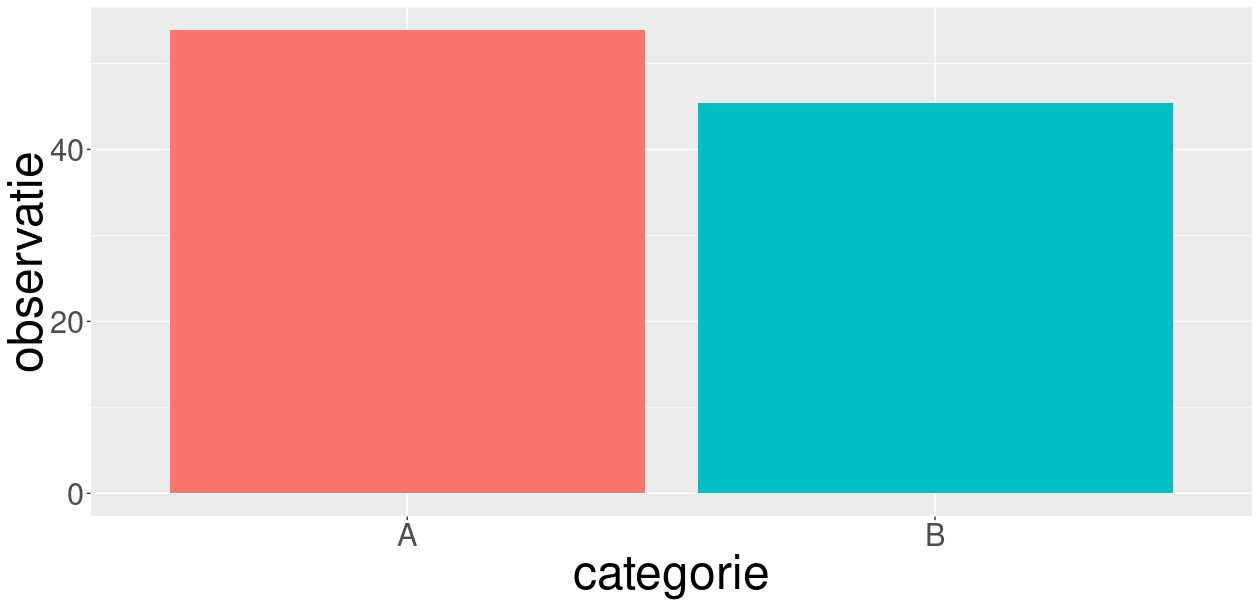
\includegraphics[width=\textwidth]{voorbeelden/barplot.png}
    \caption{Staafdiagram van gemiddelden. Dit is onvoldoende om een conclusie te trekken}
    \label{fig:barplot}
  \end{subfigure}
  \begin{subfigure}{.5\textwidth}
    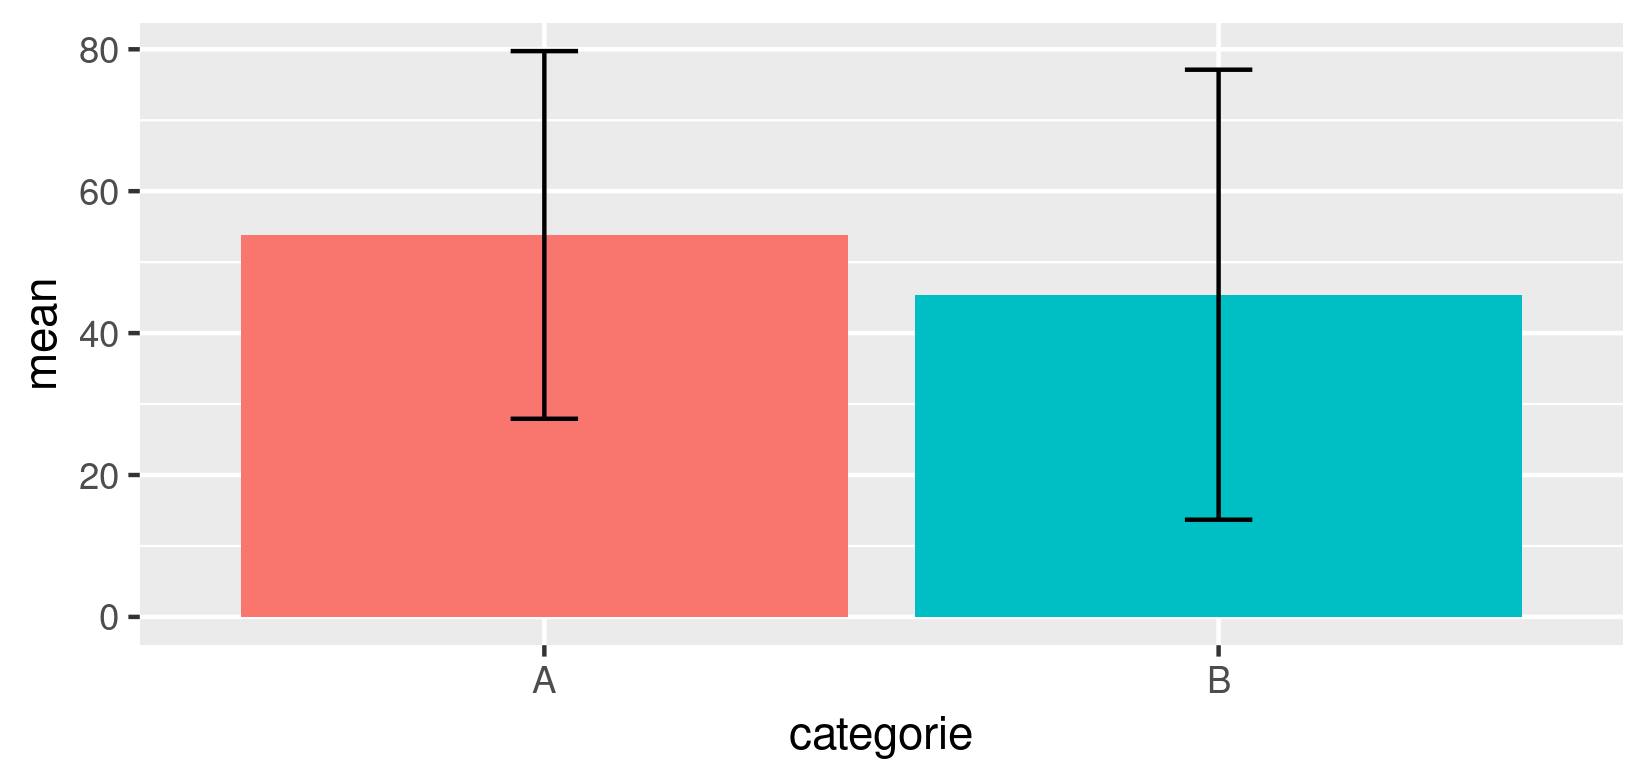
\includegraphics[width=\textwidth]{voorbeelden/barplot-errorbars.png}
    \caption{Staafdiagram met \textit{error bars} die de grootte van de steekproefstandaardafwijking voorstellen. Door de grote spreiding is het verschil tussen beide categorieën ineens veel minder uitgesproken.}
    \label{fig:barplot-errorbars}
  \end{subfigure}
  
  \begin{subfigure}{.5\textwidth}
    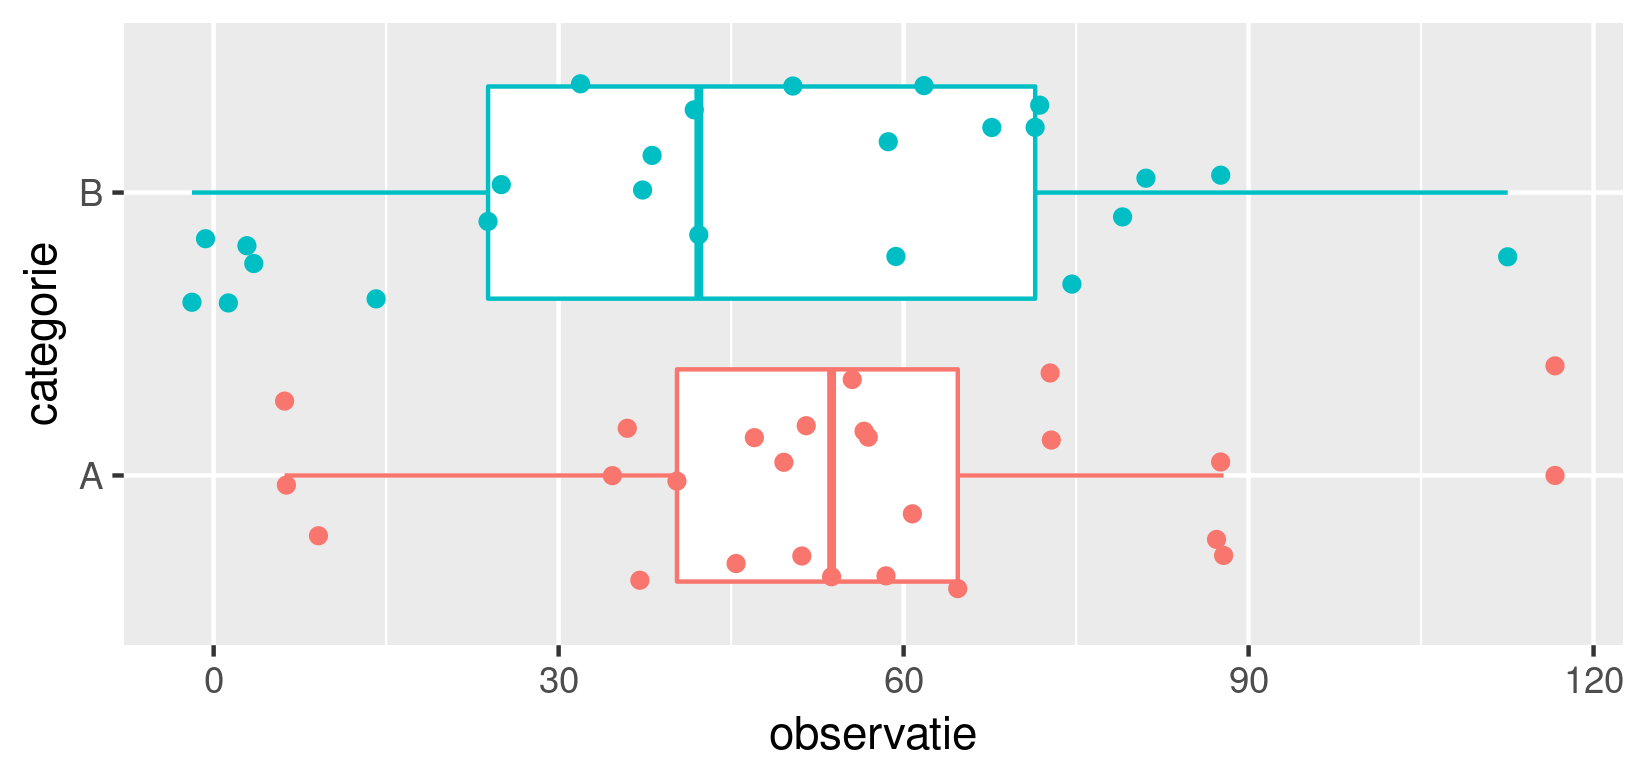
\includegraphics[width=\textwidth]{voorbeelden/boxplot-jitter.png}
    \caption{Boxplot met individuele observaties weergegeven als punten. Hiermee is de spreiding van de data nog duidelijker.}
    \label{fig:boxplot-jitter}
  \end{subfigure}
  \begin{subfigure}{.5\textwidth}
    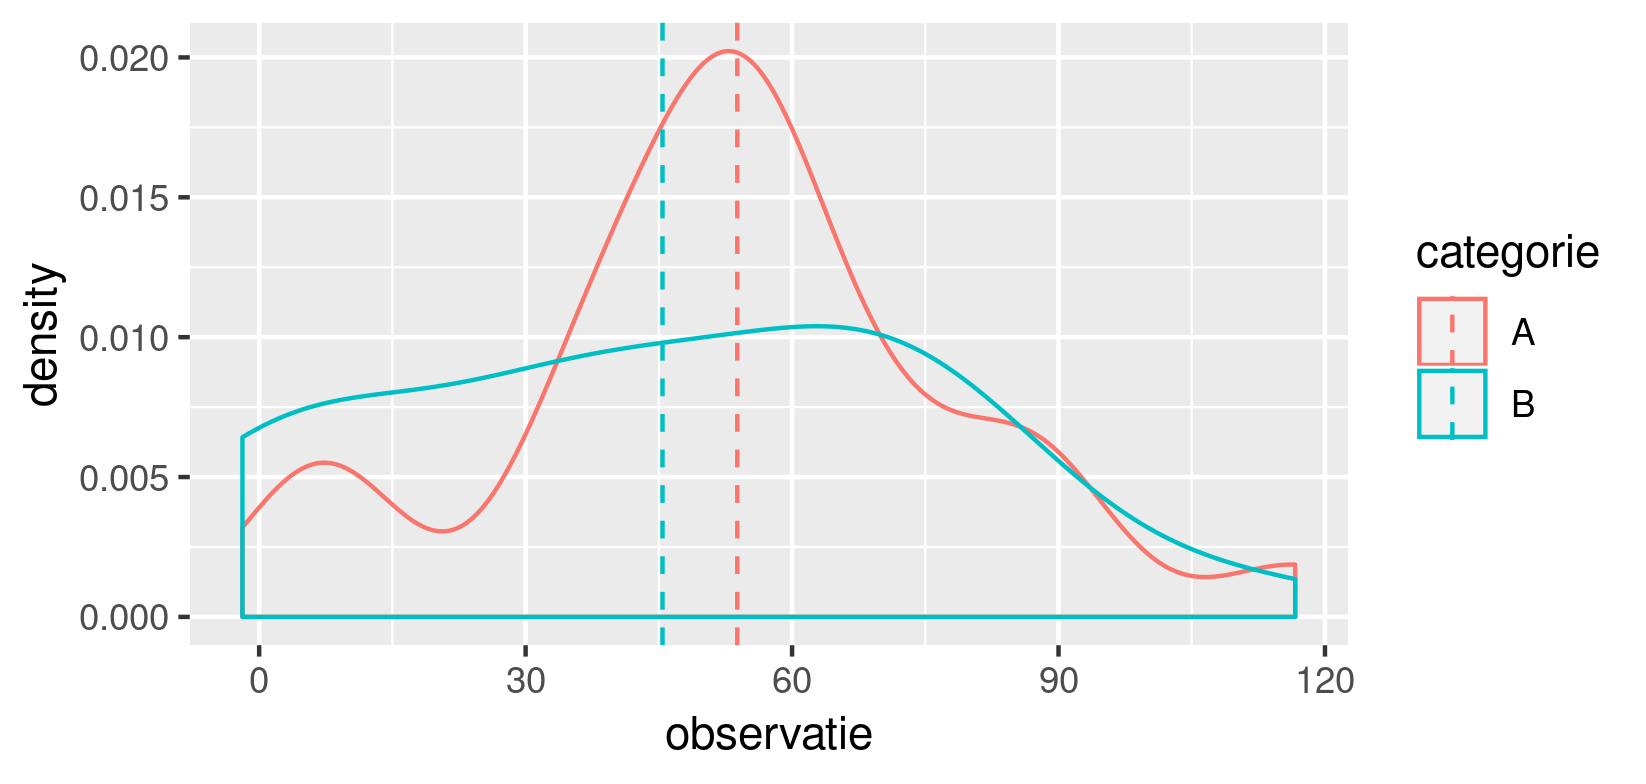
\includegraphics[width=\textwidth]{voorbeelden/density-plot.png}
    \caption{Kansdichtheid met steekproefgemiddelden aangeduid als een verticale stippellijn. Hier wordt duidelijk dat de resultaten van het experiment niet normaal verdeeld zijn. Dat maakt dat een staafdiagram met error bars eigenlijk niet geschikt is voor deze data.}
    \label{fig:density-plot}
  \end{subfigure}
  
  \caption[Visualiseren van cijfergegevens]{Verschillende manieren om dezelfde data te visualiseren.}
\end{figure}



%---------- Back matter -------------------------------------------------------
% In de bibliografie niet de bronnen uit voorbeeld.bib afdrukken. Alle bronnen
% in voorbeeld.bib moeten in het veld ``keywords'' ook de term ``voorbeeld''
% bevatten.
\printbibliography[notkeyword=voorbeeld]
\addcontentsline{toc}{chapter}{\textcolor{title}{\IfLanguageName{dutch}{Bibliografie}{Bibliography}}}

\end{document}
